\documentclass[twoside]{book}

% Packages required by doxygen
\usepackage{fixltx2e}
\usepackage{calc}
\usepackage{doxygen}
\usepackage[export]{adjustbox} % also loads graphicx
\usepackage{graphicx}
\usepackage[utf8]{inputenc}
\usepackage{makeidx}
\usepackage{multicol}
\usepackage{multirow}
\PassOptionsToPackage{warn}{textcomp}
\usepackage{textcomp}
\usepackage[nointegrals]{wasysym}
\usepackage[table]{xcolor}

% Font selection
\usepackage[T1]{fontenc}
\usepackage[scaled=.90]{helvet}
\usepackage{courier}
\usepackage{amssymb}
\usepackage{sectsty}
\renewcommand{\familydefault}{\sfdefault}
\allsectionsfont{%
  \fontseries{bc}\selectfont%
  \color{darkgray}%
}
\renewcommand{\DoxyLabelFont}{%
  \fontseries{bc}\selectfont%
  \color{darkgray}%
}
\newcommand{\+}{\discretionary{\mbox{\scriptsize$\hookleftarrow$}}{}{}}

% Page & text layout
\usepackage{geometry}
\geometry{%
  a4paper,%
  top=2.5cm,%
  bottom=2.5cm,%
  left=2.5cm,%
  right=2.5cm%
}
\tolerance=750
\hfuzz=15pt
\hbadness=750
\setlength{\emergencystretch}{15pt}
\setlength{\parindent}{0cm}
\setlength{\parskip}{0.2cm}
\makeatletter
\renewcommand{\paragraph}{%
  \@startsection{paragraph}{4}{0ex}{-1.0ex}{1.0ex}{%
    \normalfont\normalsize\bfseries\SS@parafont%
  }%
}
\renewcommand{\subparagraph}{%
  \@startsection{subparagraph}{5}{0ex}{-1.0ex}{1.0ex}{%
    \normalfont\normalsize\bfseries\SS@subparafont%
  }%
}
\makeatother

% Headers & footers
\usepackage{fancyhdr}
\pagestyle{fancyplain}
\fancyhead[LE]{\fancyplain{}{\bfseries\thepage}}
\fancyhead[CE]{\fancyplain{}{}}
\fancyhead[RE]{\fancyplain{}{\bfseries\leftmark}}
\fancyhead[LO]{\fancyplain{}{\bfseries\rightmark}}
\fancyhead[CO]{\fancyplain{}{}}
\fancyhead[RO]{\fancyplain{}{\bfseries\thepage}}
\fancyfoot[LE]{\fancyplain{}{}}
\fancyfoot[CE]{\fancyplain{}{}}
\fancyfoot[RE]{\fancyplain{}{\bfseries\scriptsize Generated on Fri Jul 24 2015 10\+:27\+:28 for rosette\+\_\+api by Doxygen }}
\fancyfoot[LO]{\fancyplain{}{\bfseries\scriptsize Generated on Fri Jul 24 2015 10\+:27\+:28 for rosette\+\_\+api by Doxygen }}
\fancyfoot[CO]{\fancyplain{}{}}
\fancyfoot[RO]{\fancyplain{}{}}
\renewcommand{\footrulewidth}{0.4pt}
\renewcommand{\chaptermark}[1]{%
  \markboth{#1}{}%
}
\renewcommand{\sectionmark}[1]{%
  \markright{\thesection\ #1}%
}

% Indices & bibliography
\usepackage{natbib}
\usepackage[titles]{tocloft}
\setcounter{tocdepth}{3}
\setcounter{secnumdepth}{5}
\makeindex

% Hyperlinks (required, but should be loaded last)
\usepackage{ifpdf}
\ifpdf
  \usepackage[pdftex,pagebackref=true]{hyperref}
\else
  \usepackage[ps2pdf,pagebackref=true]{hyperref}
\fi
\hypersetup{%
  colorlinks=true,%
  linkcolor=blue,%
  citecolor=blue,%
  unicode%
}

% Custom commands
\newcommand{\clearemptydoublepage}{%
  \newpage{\pagestyle{empty}\cleardoublepage}%
}


%===== C O N T E N T S =====

\begin{document}

% Titlepage & ToC
\hypersetup{pageanchor=false,
             bookmarks=true,
             bookmarksnumbered=true,
             pdfencoding=unicode
            }
\pagenumbering{roman}
\begin{titlepage}
\vspace*{7cm}
\begin{center}%
{\Large rosette\+\_\+api \\[1ex]\large 0.\+5.\+1 }\\
\vspace*{1cm}
{\large Generated by Doxygen 1.8.10}\\
\vspace*{0.5cm}
{\small Fri Jul 24 2015 10:27:28}\\
\end{center}
\end{titlepage}
\clearemptydoublepage
\tableofcontents
\clearemptydoublepage
\pagenumbering{arabic}
\hypersetup{pageanchor=true}

%--- Begin generated contents ---
\chapter{Namespace Index}
\section{Packages}
Here are the packages with brief descriptions (if available)\+:\begin{DoxyCompactList}
\item\contentsline{section}{\hyperlink{namespacerosette__api}{rosette\+\_\+api} }{\pageref{namespacerosette__api}}{}
\end{DoxyCompactList}

\chapter{Hierarchical Index}
\section{Class Hierarchy}
This inheritance list is sorted roughly, but not completely, alphabetically\+:\begin{DoxyCompactList}
\item \contentsline{section}{rosette\+\_\+api.\+C\+A\+P\+I}{\pageref{classrosette__api_1_1_c_a_p_i}}{}
\item Exception\begin{DoxyCompactList}
\item \contentsline{section}{rosette\+\_\+api.\+Rosette\+Exception}{\pageref{classrosette__api_1_1_rosette_exception}}{}
\end{DoxyCompactList}
\item \contentsline{section}{rosette\+\_\+api.\+Name}{\pageref{classrosette__api_1_1_name}}{}
\item \contentsline{section}{rosette\+\_\+api.\+Rosette\+File}{\pageref{classrosette__api_1_1_rosette_file}}{}
\end{DoxyCompactList}

\chapter{Class Index}
\section{Class List}
Here are the classes, structs, unions and interfaces with brief descriptions\+:\begin{DoxyCompactList}
\item\contentsline{section}{\hyperlink{classrosette__api_1_1_c_a_p_i}{rosette\+\_\+api.\+C\+A\+P\+I} \\*C\# Rosette A\+P\+I }{\pageref{classrosette__api_1_1_c_a_p_i}}{}
\item\contentsline{section}{\hyperlink{classrosette__api_1_1_name}{rosette\+\_\+api.\+Name} \\*\hyperlink{classrosette__api_1_1_name}{Name} Class }{\pageref{classrosette__api_1_1_name}}{}
\item\contentsline{section}{\hyperlink{classrosette__api_1_1_rosette_exception}{rosette\+\_\+api.\+Rosette\+Exception} \\*\hyperlink{classrosette__api_1_1_rosette_exception}{Rosette\+Exception} Class }{\pageref{classrosette__api_1_1_rosette_exception}}{}
\item\contentsline{section}{\hyperlink{classrosette__api_1_1_rosette_file}{rosette\+\_\+api.\+Rosette\+File} \\*\hyperlink{classrosette__api_1_1_rosette_file}{Rosette\+File} Class }{\pageref{classrosette__api_1_1_rosette_file}}{}
\end{DoxyCompactList}

\chapter{Namespace Documentation}
\hypertarget{namespacerosette__api}{}\section{rosette\+\_\+api Namespace Reference}
\label{namespacerosette__api}\index{rosette\+\_\+api@{rosette\+\_\+api}}
\subsection*{Classes}
\begin{DoxyCompactItemize}
\item 
class \hyperlink{classrosette__api_1_1_c_a_p_i}{C\+A\+P\+I}
\begin{DoxyCompactList}\small\item\em C\# Rosette A\+P\+I. \end{DoxyCompactList}\item 
class \hyperlink{classrosette__api_1_1_name}{Name}
\begin{DoxyCompactList}\small\item\em \hyperlink{classrosette__api_1_1_name}{Name} Class \end{DoxyCompactList}\item 
class \hyperlink{classrosette__api_1_1_rosette_exception}{Rosette\+Exception}
\begin{DoxyCompactList}\small\item\em \hyperlink{classrosette__api_1_1_rosette_exception}{Rosette\+Exception} Class \end{DoxyCompactList}\item 
class \hyperlink{classrosette__api_1_1_rosette_file}{Rosette\+File}
\begin{DoxyCompactList}\small\item\em \hyperlink{classrosette__api_1_1_rosette_file}{Rosette\+File} Class \end{DoxyCompactList}\end{DoxyCompactItemize}

\chapter{Class Documentation}
\hypertarget{classrosette__api_1_1_c_a_p_i}{}\section{rosette\+\_\+api.\+C\+A\+P\+I Class Reference}
\label{classrosette__api_1_1_c_a_p_i}\index{rosette\+\_\+api.\+C\+A\+P\+I@{rosette\+\_\+api.\+C\+A\+P\+I}}


C\# Rosette A\+P\+I.  


\subsection*{Public Member Functions}
\begin{DoxyCompactItemize}
\item 
\hyperlink{classrosette__api_1_1_c_a_p_i_ae547850ca1eedd3c8121a7a6b5ede9b7}{C\+A\+P\+I} (string user\+\_\+key, string uristring=\char`\"{}https\+://api.\+rosette.\+com/rest/v1/\char`\"{}, int max\+Retry=3, Http\+Client client=null)
\begin{DoxyCompactList}\small\item\em C\# A\+P\+I class \end{DoxyCompactList}\item 
Dictionary$<$ string, object $>$ \hyperlink{classrosette__api_1_1_c_a_p_i_a218b2b6cee592ca8869058e095df776c}{Categories} (string content=null, string language=null, string content\+Type=null, string unit=null, string content\+Uri=null)
\begin{DoxyCompactList}\small\item\em Categories \end{DoxyCompactList}\item 
Dictionary$<$ string, object $>$ \hyperlink{classrosette__api_1_1_c_a_p_i_aeac226a63205a1c7f9b0466fe542b723}{Categories} (Dictionary$<$ object, object $>$ dict)
\begin{DoxyCompactList}\small\item\em Categories \end{DoxyCompactList}\item 
Dictionary$<$ string, object $>$ \hyperlink{classrosette__api_1_1_c_a_p_i_af122d7a720ff547099f4deef3fa21d8e}{Categories} (\hyperlink{classrosette__api_1_1_rosette_file}{Rosette\+File} file)
\begin{DoxyCompactList}\small\item\em Categories \end{DoxyCompactList}\item 
Dictionary$<$ string, object $>$ \hyperlink{classrosette__api_1_1_c_a_p_i_a049d61bdb80e14925f4431a6d4709d0f}{Categories\+Info} ()
\begin{DoxyCompactList}\small\item\em Categories\+Info \end{DoxyCompactList}\item 
Dictionary$<$ string, object $>$ \hyperlink{classrosette__api_1_1_c_a_p_i_a93284702782c1b4bdde4b819870eb2da}{Entities\+Linked} (string content=null, string language=null, string content\+Type=null, string unit=null, string content\+Uri=null)
\begin{DoxyCompactList}\small\item\em Entities\+Linked \end{DoxyCompactList}\item 
Dictionary$<$ string, object $>$ \hyperlink{classrosette__api_1_1_c_a_p_i_aa6073a6b30938e088d1d23e76b50ff9f}{Entities\+Linked} (Dictionary$<$ object, object $>$ dict)
\begin{DoxyCompactList}\small\item\em Entities\+Linked \end{DoxyCompactList}\item 
Dictionary$<$ string, object $>$ \hyperlink{classrosette__api_1_1_c_a_p_i_ac8f4e67f9c37b26e3ad5a4ec2723862b}{Entities\+Linked} (\hyperlink{classrosette__api_1_1_rosette_file}{Rosette\+File} file)
\begin{DoxyCompactList}\small\item\em Entities\+Linked \end{DoxyCompactList}\item 
Dictionary$<$ string, object $>$ \hyperlink{classrosette__api_1_1_c_a_p_i_abfbd332b22b386b8da8402958a68f2d1}{Entities\+Linked\+Info} ()
\begin{DoxyCompactList}\small\item\em Entities\+Linked\+Info \end{DoxyCompactList}\item 
Dictionary$<$ string, object $>$ \hyperlink{classrosette__api_1_1_c_a_p_i_a297b73d711955c8fd36f3612c603f24b}{Entity} (string content=null, string language=null, string content\+Type=null, string unit=null, string content\+Uri=null)
\begin{DoxyCompactList}\small\item\em Entity \end{DoxyCompactList}\item 
Dictionary$<$ string, object $>$ \hyperlink{classrosette__api_1_1_c_a_p_i_a292bec5be6f2dddfcfc7a681df905e26}{Entity} (Dictionary$<$ object, object $>$ dict)
\begin{DoxyCompactList}\small\item\em Entity \end{DoxyCompactList}\item 
Dictionary$<$ string, object $>$ \hyperlink{classrosette__api_1_1_c_a_p_i_a2e38d436ce0cfff05de46671cae7a309}{Entity} (\hyperlink{classrosette__api_1_1_rosette_file}{Rosette\+File} file)
\begin{DoxyCompactList}\small\item\em Entity \end{DoxyCompactList}\item 
Dictionary$<$ string, object $>$ \hyperlink{classrosette__api_1_1_c_a_p_i_ad9bd075aca983e6dbe8b2eed3138f799}{Entity\+Info} ()
\begin{DoxyCompactList}\small\item\em Entity\+Info \end{DoxyCompactList}\item 
Dictionary$<$ string, object $>$ \hyperlink{classrosette__api_1_1_c_a_p_i_a5458accd3534ffc5c594a00bfd63551f}{Info} ()
\begin{DoxyCompactList}\small\item\em Info \end{DoxyCompactList}\item 
Dictionary$<$ string, object $>$ \hyperlink{classrosette__api_1_1_c_a_p_i_a4ed6dffb28f4abed09f7504372f7fc86}{Language} (string content=null, string language=null, string content\+Type=null, string unit=null, string content\+Uri=null)
\begin{DoxyCompactList}\small\item\em Language \end{DoxyCompactList}\item 
Dictionary$<$ string, object $>$ \hyperlink{classrosette__api_1_1_c_a_p_i_a7dc85cad4825942898152996157b0865}{Language} (Dictionary$<$ object, object $>$ dict)
\begin{DoxyCompactList}\small\item\em Language \end{DoxyCompactList}\item 
Dictionary$<$ string, object $>$ \hyperlink{classrosette__api_1_1_c_a_p_i_a83c793fc2f02dfe85b543fa17b061777}{Language} (\hyperlink{classrosette__api_1_1_rosette_file}{Rosette\+File} file)
\begin{DoxyCompactList}\small\item\em Language \end{DoxyCompactList}\item 
Dictionary$<$ string, object $>$ \hyperlink{classrosette__api_1_1_c_a_p_i_a2dcf183afd4f5b7511a17efa5c42ffda}{Language\+Info} ()
\begin{DoxyCompactList}\small\item\em Language\+Info \end{DoxyCompactList}\item 
Dictionary$<$ string, object $>$ \hyperlink{classrosette__api_1_1_c_a_p_i_a8ffe39cfe01a07dc1b67f2bc76b1f92d}{Morphology} (string content=null, string language=null, string content\+Type=null, string unit=null, string content\+Uri=null, string feature=\char`\"{}complete\char`\"{})
\begin{DoxyCompactList}\small\item\em Morphology \end{DoxyCompactList}\item 
Dictionary$<$ string, object $>$ \hyperlink{classrosette__api_1_1_c_a_p_i_a578e155f77e3baa51c56d38724567855}{Morphology} (Dictionary$<$ object, object $>$ dict, string feature=\char`\"{}complete\char`\"{})
\begin{DoxyCompactList}\small\item\em Morphology \end{DoxyCompactList}\item 
Dictionary$<$ string, object $>$ \hyperlink{classrosette__api_1_1_c_a_p_i_a57a341be212d74390da90a31c7b65e94}{Morphology} (\hyperlink{classrosette__api_1_1_rosette_file}{Rosette\+File} file, string feature=\char`\"{}complete\char`\"{})
\begin{DoxyCompactList}\small\item\em Morphology \end{DoxyCompactList}\item 
Dictionary$<$ string, object $>$ \hyperlink{classrosette__api_1_1_c_a_p_i_a4348a323976b5686dc6fa613d085be86}{Matched\+Name} (\hyperlink{classrosette__api_1_1_name}{Name} n1, \hyperlink{classrosette__api_1_1_name}{Name} n2)
\begin{DoxyCompactList}\small\item\em Matched\+Name \end{DoxyCompactList}\item 
Dictionary$<$ string, object $>$ \hyperlink{classrosette__api_1_1_c_a_p_i_a379a8a3cb7b34a9f1a8e4e50f06f8eeb}{Matched\+Name} (Dictionary$<$ object, object $>$ dict)
\begin{DoxyCompactList}\small\item\em Matched\+Name \end{DoxyCompactList}\item 
Dictionary$<$ string, object $>$ \hyperlink{classrosette__api_1_1_c_a_p_i_a2da4ec1037afca2ca38624565dbb3cf5}{Matched\+Name\+Info} ()
\begin{DoxyCompactList}\small\item\em Matched\+Name\+Info \end{DoxyCompactList}\item 
Dictionary$<$ string, object $>$ \hyperlink{classrosette__api_1_1_c_a_p_i_ac2cd22efe9ad2fd8eaaf990e278ed6f2}{Ping} ()
\begin{DoxyCompactList}\small\item\em Ping (G\+E\+T)Ping Endpoint\+: Pings Rosette A\+P\+I for a response indicting that the service is available \end{DoxyCompactList}\item 
Dictionary$<$ string, object $>$ \hyperlink{classrosette__api_1_1_c_a_p_i_ae2693ce28755a76c93537e68914b5cb2}{Sentences} (string content=null, string language=null, string content\+Type=null, string unit=null, string content\+Uri=null)
\begin{DoxyCompactList}\small\item\em Sentences \end{DoxyCompactList}\item 
Dictionary$<$ string, object $>$ \hyperlink{classrosette__api_1_1_c_a_p_i_acd9b4b1b5deaf2d5d85464fb4ac7b135}{Sentences} (Dictionary$<$ object, object $>$ dict)
\begin{DoxyCompactList}\small\item\em Sentences \end{DoxyCompactList}\item 
Dictionary$<$ string, object $>$ \hyperlink{classrosette__api_1_1_c_a_p_i_ac8c2831cfaa5fcd727f4eadcbaea567d}{Sentences} (\hyperlink{classrosette__api_1_1_rosette_file}{Rosette\+File} file)
\begin{DoxyCompactList}\small\item\em Sentences \end{DoxyCompactList}\item 
Dictionary$<$ string, object $>$ \hyperlink{classrosette__api_1_1_c_a_p_i_aad62971ec700b73052693fdaa2133939}{Sentiment} (string content=null, string language=null, string content\+Type=null, string unit=null, string content\+Uri=null)
\begin{DoxyCompactList}\small\item\em Sentiment \end{DoxyCompactList}\item 
Dictionary$<$ string, object $>$ \hyperlink{classrosette__api_1_1_c_a_p_i_a22f6c14f1e484355a32af2de6cc9ae57}{Sentiment} (Dictionary$<$ object, object $>$ dict)
\begin{DoxyCompactList}\small\item\em Sentiment \end{DoxyCompactList}\item 
Dictionary$<$ string, object $>$ \hyperlink{classrosette__api_1_1_c_a_p_i_a35ab561303c1d997fb22635942523a6c}{Sentiment} (\hyperlink{classrosette__api_1_1_rosette_file}{Rosette\+File} file)
\begin{DoxyCompactList}\small\item\em Sentiment \end{DoxyCompactList}\item 
Dictionary$<$ string, object $>$ \hyperlink{classrosette__api_1_1_c_a_p_i_aef053823a3490b2cc15b4aa040d72508}{Sentiment\+Info} ()
\begin{DoxyCompactList}\small\item\em Sentiment\+Info \end{DoxyCompactList}\item 
Dictionary$<$ string, object $>$ \hyperlink{classrosette__api_1_1_c_a_p_i_a0bea36c60aaf9271927b81e38613a401}{Tokens} (string content=null, string language=null, string content\+Type=null, string unit=null, string content\+Uri=null)
\begin{DoxyCompactList}\small\item\em Tokens \end{DoxyCompactList}\item 
Dictionary$<$ string, object $>$ \hyperlink{classrosette__api_1_1_c_a_p_i_a2d1fabbeff31fb0e57527b7729255fed}{Tokens} (Dictionary$<$ object, object $>$ dict)
\begin{DoxyCompactList}\small\item\em Tokens \end{DoxyCompactList}\item 
Dictionary$<$ string, object $>$ \hyperlink{classrosette__api_1_1_c_a_p_i_a7e66399baa757fe6baa676419660fdd8}{Tokens} (\hyperlink{classrosette__api_1_1_rosette_file}{Rosette\+File} file)
\begin{DoxyCompactList}\small\item\em Tokens \end{DoxyCompactList}\item 
Dictionary$<$ string, object $>$ \hyperlink{classrosette__api_1_1_c_a_p_i_a58db505790eb9d805650df07b0850b04}{Translated\+Name} (string name, string source\+Language\+Of\+Use=null, string source\+Script=null, string target\+Language=null, string target\+Script=null, string target\+Scheme=null, string source\+Language\+Of\+Origin=null, string entity\+Type=null)
\begin{DoxyCompactList}\small\item\em Translated\+Name \end{DoxyCompactList}\item 
Dictionary$<$ string, object $>$ \hyperlink{classrosette__api_1_1_c_a_p_i_a705a8033ee7c8da35e1544de53137084}{Translated\+Name} (Dictionary$<$ object, object $>$ dict)
\begin{DoxyCompactList}\small\item\em Translated\+Name \end{DoxyCompactList}\item 
Dictionary$<$ string, object $>$ \hyperlink{classrosette__api_1_1_c_a_p_i_af5e226e8bbf466846ffb4e9786821fcd}{Translated\+Name\+Info} ()
\begin{DoxyCompactList}\small\item\em Translated\+Name\+Info \end{DoxyCompactList}\end{DoxyCompactItemize}
\subsection*{Properties}
\begin{DoxyCompactItemize}
\item 
string \hyperlink{classrosette__api_1_1_c_a_p_i_a841f1b659a19158a503657d71020acba}{User\+Key}\hspace{0.3cm}{\ttfamily  \mbox{[}get, set\mbox{]}}
\begin{DoxyCompactList}\small\item\em User\+Key \end{DoxyCompactList}\item 
string \hyperlink{classrosette__api_1_1_c_a_p_i_a3c358533f274d3cd22d789d943a57e68}{U\+R\+Istring}\hspace{0.3cm}{\ttfamily  \mbox{[}get, set\mbox{]}}
\begin{DoxyCompactList}\small\item\em U\+R\+Istring \end{DoxyCompactList}\item 
int \hyperlink{classrosette__api_1_1_c_a_p_i_a62b4bd9343e43477f512ada376d4896d}{Max\+Retry}\hspace{0.3cm}{\ttfamily  \mbox{[}get, set\mbox{]}}
\begin{DoxyCompactList}\small\item\em Max\+Retry \end{DoxyCompactList}\item 
Http\+Client \hyperlink{classrosette__api_1_1_c_a_p_i_adb40d6828661d95567d124a2a57852d5}{Client}\hspace{0.3cm}{\ttfamily  \mbox{[}get, set\mbox{]}}
\begin{DoxyCompactList}\small\item\em Client \end{DoxyCompactList}\item 
bool \hyperlink{classrosette__api_1_1_c_a_p_i_a16e8da8b7074a7d92505c623945f5b6e}{Debug}\hspace{0.3cm}{\ttfamily  \mbox{[}get, set\mbox{]}}
\begin{DoxyCompactList}\small\item\em Debug \end{DoxyCompactList}\item 
int \hyperlink{classrosette__api_1_1_c_a_p_i_a3e204eb9849f713e523e744e2ca5a1f1}{Timeout}\hspace{0.3cm}{\ttfamily  \mbox{[}get, set\mbox{]}}
\begin{DoxyCompactList}\small\item\em Timeout \end{DoxyCompactList}\end{DoxyCompactItemize}


\subsection{Detailed Description}
C\# Rosette A\+P\+I. 

Primary class for interfacing with the Rosette A\+P\+I \begin{DoxyCopyright}{Copyright}
2014-\/2015 Basis Technology Corporation. Licensed under the Apache License, Version 2.\+0 (the \char`\"{}\+License\char`\"{}); you may not use this file except in compliance with the License. You may obtain a copy of the License at \href{http://www.apache.org/licenses/LICENSE-2.0}{\tt http\+://www.\+apache.\+org/licenses/\+L\+I\+C\+E\+N\+S\+E-\/2.\+0} Unless required by applicable law or agreed to in writing, software distributed under the License is distributed on an \char`\"{}\+A\+S I\+S\char`\"{} B\+A\+S\+I\+S, W\+I\+T\+H\+O\+U\+T W\+A\+R\+R\+A\+N\+T\+I\+E\+S O\+R C\+O\+N\+D\+I\+T\+I\+O\+N\+S O\+F A\+N\+Y K\+I\+N\+D, either express or implied. See the License for the specific language governing permissions and limitations under the License. 
\end{DoxyCopyright}


\subsection{Constructor \& Destructor Documentation}
\hypertarget{classrosette__api_1_1_c_a_p_i_ae547850ca1eedd3c8121a7a6b5ede9b7}{}\index{rosette\+\_\+api\+::\+C\+A\+P\+I@{rosette\+\_\+api\+::\+C\+A\+P\+I}!C\+A\+P\+I@{C\+A\+P\+I}}
\index{C\+A\+P\+I@{C\+A\+P\+I}!rosette\+\_\+api\+::\+C\+A\+P\+I@{rosette\+\_\+api\+::\+C\+A\+P\+I}}
\subsubsection[{C\+A\+P\+I(string user\+\_\+key, string uristring=""https\+://api.\+rosette.\+com/rest/v1/"", int max\+Retry=3, Http\+Client client=null)}]{\setlength{\rightskip}{0pt plus 5cm}rosette\+\_\+api.\+C\+A\+P\+I.\+C\+A\+P\+I (
\begin{DoxyParamCaption}
\item[{string}]{user\+\_\+key, }
\item[{string}]{uristring = {\ttfamily \char`\"{}https\+://api.rosette.com/rest/v1/\char`\"{}}, }
\item[{int}]{max\+Retry = {\ttfamily 3}, }
\item[{Http\+Client}]{client = {\ttfamily null}}
\end{DoxyParamCaption}
)}\label{classrosette__api_1_1_c_a_p_i_ae547850ca1eedd3c8121a7a6b5ede9b7}


C\# A\+P\+I class 

Rosette Python Client Binding A\+P\+I; representation of a Rosette server. Instance methods of the C\# A\+P\+I provide communication with specific Rosette server endpoints. Requires user\+\_\+key to start and has 3 additional parameters to be specified. Will run a Version Check against the Rosette Server. If the version check fails, a \hyperlink{classrosette__api_1_1_rosette_exception}{Rosette\+Exception} will be thrown. 


\begin{DoxyParams}{Parameters}
{\em user\+\_\+key} & string\+: A\+P\+I key required by the Rosette server to allow access to endpoints\\
\hline
{\em uristring} & (string, optional)\+: Base U\+R\+L for the Http\+Client requests. If none is given, will use the default A\+P\+I U\+R\+I\\
\hline
{\em max\+Retry} & (int, optional)\+: Maximum number of times to retry a request on Http\+Response error. Default is 3 times.\\
\hline
{\em client} & (Http\+Client, optional)\+: Forces the A\+P\+I to use a custom Http\+Client.\\
\hline
\end{DoxyParams}


\subsection{Member Function Documentation}
\hypertarget{classrosette__api_1_1_c_a_p_i_a218b2b6cee592ca8869058e095df776c}{}\index{rosette\+\_\+api\+::\+C\+A\+P\+I@{rosette\+\_\+api\+::\+C\+A\+P\+I}!Categories@{Categories}}
\index{Categories@{Categories}!rosette\+\_\+api\+::\+C\+A\+P\+I@{rosette\+\_\+api\+::\+C\+A\+P\+I}}
\subsubsection[{Categories(string content=null, string language=null, string content\+Type=null, string unit=null, string content\+Uri=null)}]{\setlength{\rightskip}{0pt plus 5cm}Dictionary$<$string, object$>$ rosette\+\_\+api.\+C\+A\+P\+I.\+Categories (
\begin{DoxyParamCaption}
\item[{string}]{content = {\ttfamily null}, }
\item[{string}]{language = {\ttfamily null}, }
\item[{string}]{content\+Type = {\ttfamily null}, }
\item[{string}]{unit = {\ttfamily null}, }
\item[{string}]{content\+Uri = {\ttfamily null}}
\end{DoxyParamCaption}
)}\label{classrosette__api_1_1_c_a_p_i_a218b2b6cee592ca8869058e095df776c}


Categories 

(P\+O\+S\+T)Categories Endpoint\+: Returns an ordered list of categories identified in the input. The categories are Tier 1 contextual categories defined in the Q\+A\+G Taxonomy. 


\begin{DoxyParams}{Parameters}
{\em content} & (string, optional)\+: Input to process (J\+S\+O\+N string or base64 encoding of non-\/\+J\+S\+O\+N string)\\
\hline
{\em language} & (string, optional)\+: Language\+: I\+S\+O 639-\/3 code (ignored for the /language endpoint)\\
\hline
{\em content\+Type} & (string, optional)\+: M\+I\+M\+E type of the input (required for base64 content; if content type is unknown, set to \char`\"{}application/octet-\/stream\char`\"{})\\
\hline
{\em unit} & (string, optional)\+: Input unit\+: \char`\"{}doc\char`\"{} (document, the default) or \char`\"{}sentence\char`\"{}\\
\hline
{\em content\+Uri} & (string, optional)\+: U\+R\+I to accessible content (content and content\+Uri are mutually exclusive)\\
\hline
\end{DoxyParams}
\begin{DoxyReturn}{Returns}
Dictionary$<$string, object$>$\+: Dictionary containing the results of the request. The response is the contextual categories identified in the input. 
\end{DoxyReturn}
\hypertarget{classrosette__api_1_1_c_a_p_i_aeac226a63205a1c7f9b0466fe542b723}{}\index{rosette\+\_\+api\+::\+C\+A\+P\+I@{rosette\+\_\+api\+::\+C\+A\+P\+I}!Categories@{Categories}}
\index{Categories@{Categories}!rosette\+\_\+api\+::\+C\+A\+P\+I@{rosette\+\_\+api\+::\+C\+A\+P\+I}}
\subsubsection[{Categories(\+Dictionary$<$ object, object $>$ dict)}]{\setlength{\rightskip}{0pt plus 5cm}Dictionary$<$string, object$>$ rosette\+\_\+api.\+C\+A\+P\+I.\+Categories (
\begin{DoxyParamCaption}
\item[{Dictionary$<$ object, object $>$}]{dict}
\end{DoxyParamCaption}
)}\label{classrosette__api_1_1_c_a_p_i_aeac226a63205a1c7f9b0466fe542b723}


Categories 

(P\+O\+S\+T)Categories Endpoint\+: Returns an ordered list of categories identified in the input. The categories are Tier 1 contextual categories defined in the Q\+A\+G Taxonomy. 


\begin{DoxyParams}{Parameters}
{\em dict} & Dictionary$<$object, object$>$\+: Dictionary containing parameters as (key,value) pairs\\
\hline
\end{DoxyParams}
\begin{DoxyReturn}{Returns}
Dictionary$<$string, object$>$\+: Dictionary containing the results of the request. The response is the contextual categories identified in the input. 
\end{DoxyReturn}
\hypertarget{classrosette__api_1_1_c_a_p_i_af122d7a720ff547099f4deef3fa21d8e}{}\index{rosette\+\_\+api\+::\+C\+A\+P\+I@{rosette\+\_\+api\+::\+C\+A\+P\+I}!Categories@{Categories}}
\index{Categories@{Categories}!rosette\+\_\+api\+::\+C\+A\+P\+I@{rosette\+\_\+api\+::\+C\+A\+P\+I}}
\subsubsection[{Categories(\+Rosette\+File file)}]{\setlength{\rightskip}{0pt plus 5cm}Dictionary$<$string, object$>$ rosette\+\_\+api.\+C\+A\+P\+I.\+Categories (
\begin{DoxyParamCaption}
\item[{{\bf Rosette\+File}}]{file}
\end{DoxyParamCaption}
)}\label{classrosette__api_1_1_c_a_p_i_af122d7a720ff547099f4deef3fa21d8e}


Categories 

(P\+O\+S\+T)Categories Endpoint\+: Returns an ordered list of categories identified in the input. The categories are Tier 1 contextual categories defined in the Q\+A\+G Taxonomy. 


\begin{DoxyParams}{Parameters}
{\em file} & \hyperlink{classrosette__api_1_1_rosette_file}{Rosette\+File}\+: \hyperlink{classrosette__api_1_1_rosette_file}{Rosette\+File} Object containing the file (and possibly options) to upload\\
\hline
\end{DoxyParams}
\begin{DoxyReturn}{Returns}
Dictionary$<$string, object$>$\+: Dictionary containing the results of the request. The response is the contextual categories identified in the input. 
\end{DoxyReturn}
\hypertarget{classrosette__api_1_1_c_a_p_i_a049d61bdb80e14925f4431a6d4709d0f}{}\index{rosette\+\_\+api\+::\+C\+A\+P\+I@{rosette\+\_\+api\+::\+C\+A\+P\+I}!Categories\+Info@{Categories\+Info}}
\index{Categories\+Info@{Categories\+Info}!rosette\+\_\+api\+::\+C\+A\+P\+I@{rosette\+\_\+api\+::\+C\+A\+P\+I}}
\subsubsection[{Categories\+Info()}]{\setlength{\rightskip}{0pt plus 5cm}Dictionary$<$string, object$>$ rosette\+\_\+api.\+C\+A\+P\+I.\+Categories\+Info (
\begin{DoxyParamCaption}
{}
\end{DoxyParamCaption}
)}\label{classrosette__api_1_1_c_a_p_i_a049d61bdb80e14925f4431a6d4709d0f}


Categories\+Info 

(G\+E\+T\+Categories\+Info Endpoint\+: Response is a J\+S\+O\+N string with request id, version, build info, and support (null for now). 

\begin{DoxyReturn}{Returns}
Dictionary$<$string, object$>$\+: Dictionary containing the results of the info G\+E\+T.
\end{DoxyReturn}
\hypertarget{classrosette__api_1_1_c_a_p_i_a93284702782c1b4bdde4b819870eb2da}{}\index{rosette\+\_\+api\+::\+C\+A\+P\+I@{rosette\+\_\+api\+::\+C\+A\+P\+I}!Entities\+Linked@{Entities\+Linked}}
\index{Entities\+Linked@{Entities\+Linked}!rosette\+\_\+api\+::\+C\+A\+P\+I@{rosette\+\_\+api\+::\+C\+A\+P\+I}}
\subsubsection[{Entities\+Linked(string content=null, string language=null, string content\+Type=null, string unit=null, string content\+Uri=null)}]{\setlength{\rightskip}{0pt plus 5cm}Dictionary$<$string, object$>$ rosette\+\_\+api.\+C\+A\+P\+I.\+Entities\+Linked (
\begin{DoxyParamCaption}
\item[{string}]{content = {\ttfamily null}, }
\item[{string}]{language = {\ttfamily null}, }
\item[{string}]{content\+Type = {\ttfamily null}, }
\item[{string}]{unit = {\ttfamily null}, }
\item[{string}]{content\+Uri = {\ttfamily null}}
\end{DoxyParamCaption}
)}\label{classrosette__api_1_1_c_a_p_i_a93284702782c1b4bdde4b819870eb2da}


Entities\+Linked 

(P\+O\+S\+T)Entities\+Linked Endpoint\+: Links entities in the input to entities in the knowledge base. 


\begin{DoxyParams}{Parameters}
{\em content} & (string, optional)\+: Input to process (J\+S\+O\+N string or base64 encoding of non-\/\+J\+S\+O\+N string)\\
\hline
{\em language} & (string, optional)\+: Language\+: I\+S\+O 639-\/3 code (ignored for the /language endpoint)\\
\hline
{\em content\+Type} & (string, optional)\+: M\+I\+M\+E type of the input (required for base64 content; if content type is unknown, set to \char`\"{}application/octet-\/stream\char`\"{})\\
\hline
{\em unit} & (string, optional)\+: Input unit\+: \char`\"{}doc\char`\"{} (document, the default) or \char`\"{}sentence\char`\"{}\\
\hline
{\em content\+Uri} & (string, optional)\+: U\+R\+I to accessible content (content and content\+Uri are mutually exclusive)\\
\hline
\end{DoxyParams}
\begin{DoxyReturn}{Returns}
Dictionary$<$string, object$>$\+: Dictionary containing the results of the request. The response identifies the entities in the input that have been linked to entities in the knowledge base. Each entity includes an entity id (from the knowledge base), a chain id (all instances of the same entity share a chain id), the mention (entity text from the input), and confidence associated with the linking. 
\end{DoxyReturn}
\hypertarget{classrosette__api_1_1_c_a_p_i_aa6073a6b30938e088d1d23e76b50ff9f}{}\index{rosette\+\_\+api\+::\+C\+A\+P\+I@{rosette\+\_\+api\+::\+C\+A\+P\+I}!Entities\+Linked@{Entities\+Linked}}
\index{Entities\+Linked@{Entities\+Linked}!rosette\+\_\+api\+::\+C\+A\+P\+I@{rosette\+\_\+api\+::\+C\+A\+P\+I}}
\subsubsection[{Entities\+Linked(\+Dictionary$<$ object, object $>$ dict)}]{\setlength{\rightskip}{0pt plus 5cm}Dictionary$<$string, object$>$ rosette\+\_\+api.\+C\+A\+P\+I.\+Entities\+Linked (
\begin{DoxyParamCaption}
\item[{Dictionary$<$ object, object $>$}]{dict}
\end{DoxyParamCaption}
)}\label{classrosette__api_1_1_c_a_p_i_aa6073a6b30938e088d1d23e76b50ff9f}


Entities\+Linked 

(P\+O\+S\+T)Entities\+Linked Endpoint\+: Links entities in the input to entities in the knowledge base. 


\begin{DoxyParams}{Parameters}
{\em dict} & Dictionary$<$object, object$>$\+: Dictionary containing parameters as (key,value) pairs\\
\hline
\end{DoxyParams}
\begin{DoxyReturn}{Returns}
Dictionary$<$string, object$>$\+: Dictionary containing the results of the request. The response identifies the entities in the input that have been linked to entities in the knowledge base. Each entity includes an entity id (from the knowledge base), a chain id (all instances of the same entity share a chain id), the mention (entity text from the input), and confidence associated with the linking. 
\end{DoxyReturn}
\hypertarget{classrosette__api_1_1_c_a_p_i_ac8f4e67f9c37b26e3ad5a4ec2723862b}{}\index{rosette\+\_\+api\+::\+C\+A\+P\+I@{rosette\+\_\+api\+::\+C\+A\+P\+I}!Entities\+Linked@{Entities\+Linked}}
\index{Entities\+Linked@{Entities\+Linked}!rosette\+\_\+api\+::\+C\+A\+P\+I@{rosette\+\_\+api\+::\+C\+A\+P\+I}}
\subsubsection[{Entities\+Linked(\+Rosette\+File file)}]{\setlength{\rightskip}{0pt plus 5cm}Dictionary$<$string, object$>$ rosette\+\_\+api.\+C\+A\+P\+I.\+Entities\+Linked (
\begin{DoxyParamCaption}
\item[{{\bf Rosette\+File}}]{file}
\end{DoxyParamCaption}
)}\label{classrosette__api_1_1_c_a_p_i_ac8f4e67f9c37b26e3ad5a4ec2723862b}


Entities\+Linked 

(P\+O\+S\+T)Entities\+Linked Endpoint\+: Links entities in the input to entities in the knowledge base. 


\begin{DoxyParams}{Parameters}
{\em file} & \hyperlink{classrosette__api_1_1_rosette_file}{Rosette\+File}\+: \hyperlink{classrosette__api_1_1_rosette_file}{Rosette\+File} Object containing the file (and possibly options) to upload\\
\hline
\end{DoxyParams}
\begin{DoxyReturn}{Returns}
Dictionary$<$string, object$>$\+: Dictionary containing the results of the request. The response identifies the entities in the input that have been linked to entities in the knowledge base. Each entity includes an entity id (from the knowledge base), a chain id (all instances of the same entity share a chain id), the mention (entity text from the input), and confidence associated with the linking. 
\end{DoxyReturn}
\hypertarget{classrosette__api_1_1_c_a_p_i_abfbd332b22b386b8da8402958a68f2d1}{}\index{rosette\+\_\+api\+::\+C\+A\+P\+I@{rosette\+\_\+api\+::\+C\+A\+P\+I}!Entities\+Linked\+Info@{Entities\+Linked\+Info}}
\index{Entities\+Linked\+Info@{Entities\+Linked\+Info}!rosette\+\_\+api\+::\+C\+A\+P\+I@{rosette\+\_\+api\+::\+C\+A\+P\+I}}
\subsubsection[{Entities\+Linked\+Info()}]{\setlength{\rightskip}{0pt plus 5cm}Dictionary$<$string, object$>$ rosette\+\_\+api.\+C\+A\+P\+I.\+Entities\+Linked\+Info (
\begin{DoxyParamCaption}
{}
\end{DoxyParamCaption}
)}\label{classrosette__api_1_1_c_a_p_i_abfbd332b22b386b8da8402958a68f2d1}


Entities\+Linked\+Info 

(G\+E\+T)Entities\+Linked\+Info Endpoint\+: Response is a J\+S\+O\+N string with request id, version, build info, and support (null for now). 

\begin{DoxyReturn}{Returns}
Dictionary$<$string, object$>$\+: Dictionary containing the results of the info G\+E\+T.
\end{DoxyReturn}
\hypertarget{classrosette__api_1_1_c_a_p_i_a297b73d711955c8fd36f3612c603f24b}{}\index{rosette\+\_\+api\+::\+C\+A\+P\+I@{rosette\+\_\+api\+::\+C\+A\+P\+I}!Entity@{Entity}}
\index{Entity@{Entity}!rosette\+\_\+api\+::\+C\+A\+P\+I@{rosette\+\_\+api\+::\+C\+A\+P\+I}}
\subsubsection[{Entity(string content=null, string language=null, string content\+Type=null, string unit=null, string content\+Uri=null)}]{\setlength{\rightskip}{0pt plus 5cm}Dictionary$<$string, object$>$ rosette\+\_\+api.\+C\+A\+P\+I.\+Entity (
\begin{DoxyParamCaption}
\item[{string}]{content = {\ttfamily null}, }
\item[{string}]{language = {\ttfamily null}, }
\item[{string}]{content\+Type = {\ttfamily null}, }
\item[{string}]{unit = {\ttfamily null}, }
\item[{string}]{content\+Uri = {\ttfamily null}}
\end{DoxyParamCaption}
)}\label{classrosette__api_1_1_c_a_p_i_a297b73d711955c8fd36f3612c603f24b}


Entity 

(P\+O\+S\+T)Entity Endpoint\+: Returns each entity extracted from the input. 


\begin{DoxyParams}{Parameters}
{\em content} & (string, optional)\+: Input to process (J\+S\+O\+N string or base64 encoding of non-\/\+J\+S\+O\+N string)\\
\hline
{\em language} & (string, optional)\+: Language\+: I\+S\+O 639-\/3 code (ignored for the /language endpoint)\\
\hline
{\em content\+Type} & (string, optional)\+: M\+I\+M\+E type of the input (required for base64 content; if content type is unknown, set to \char`\"{}application/octet-\/stream\char`\"{})\\
\hline
{\em unit} & (string, optional)\+: Input unit\+: \char`\"{}doc\char`\"{} (document, the default) or \char`\"{}sentence\char`\"{}\\
\hline
{\em content\+Uri} & (string, optional)\+: U\+R\+I to accessible content (content and content\+Uri are mutually exclusive)\\
\hline
\end{DoxyParams}
\begin{DoxyReturn}{Returns}
Dictionary$<$string, object$>$\+: Dictionary containing the results of the request. The response is a list of extracted entities. Each entity includes chain I\+D (all instances of the same entity share a chain id), mention (entity text in the input), normalized text (the most complete form of this entity that appears in the input), count (how many times this entity appears in the input), and the confidence associated with the extraction. 
\end{DoxyReturn}
\hypertarget{classrosette__api_1_1_c_a_p_i_a292bec5be6f2dddfcfc7a681df905e26}{}\index{rosette\+\_\+api\+::\+C\+A\+P\+I@{rosette\+\_\+api\+::\+C\+A\+P\+I}!Entity@{Entity}}
\index{Entity@{Entity}!rosette\+\_\+api\+::\+C\+A\+P\+I@{rosette\+\_\+api\+::\+C\+A\+P\+I}}
\subsubsection[{Entity(\+Dictionary$<$ object, object $>$ dict)}]{\setlength{\rightskip}{0pt plus 5cm}Dictionary$<$string, object$>$ rosette\+\_\+api.\+C\+A\+P\+I.\+Entity (
\begin{DoxyParamCaption}
\item[{Dictionary$<$ object, object $>$}]{dict}
\end{DoxyParamCaption}
)}\label{classrosette__api_1_1_c_a_p_i_a292bec5be6f2dddfcfc7a681df905e26}


Entity 

(P\+O\+S\+T)Entity Endpoint\+: Returns each entity extracted from the input. 


\begin{DoxyParams}{Parameters}
{\em dict} & Dictionary$<$object, object$>$\+: Dictionary containing parameters as (key,value) pairs\\
\hline
\end{DoxyParams}
\begin{DoxyReturn}{Returns}
Dictionary$<$string, object$>$\+: Dictionary containing the results of the request. The response is a list of extracted entities. Each entity includes chain I\+D (all instances of the same entity share a chain id), mention (entity text in the input), normalized text (the most complete form of this entity that appears in the input), count (how many times this entity appears in the input), and the confidence associated with the extraction. 
\end{DoxyReturn}
\hypertarget{classrosette__api_1_1_c_a_p_i_a2e38d436ce0cfff05de46671cae7a309}{}\index{rosette\+\_\+api\+::\+C\+A\+P\+I@{rosette\+\_\+api\+::\+C\+A\+P\+I}!Entity@{Entity}}
\index{Entity@{Entity}!rosette\+\_\+api\+::\+C\+A\+P\+I@{rosette\+\_\+api\+::\+C\+A\+P\+I}}
\subsubsection[{Entity(\+Rosette\+File file)}]{\setlength{\rightskip}{0pt plus 5cm}Dictionary$<$string, object$>$ rosette\+\_\+api.\+C\+A\+P\+I.\+Entity (
\begin{DoxyParamCaption}
\item[{{\bf Rosette\+File}}]{file}
\end{DoxyParamCaption}
)}\label{classrosette__api_1_1_c_a_p_i_a2e38d436ce0cfff05de46671cae7a309}


Entity 

(P\+O\+S\+T)Entity Endpoint\+: Returns each entity extracted from the input. 


\begin{DoxyParams}{Parameters}
{\em file} & \hyperlink{classrosette__api_1_1_rosette_file}{Rosette\+File}\+: \hyperlink{classrosette__api_1_1_rosette_file}{Rosette\+File} Object containing the file (and possibly options) to upload\\
\hline
\end{DoxyParams}
\begin{DoxyReturn}{Returns}
Dictionary$<$string, object$>$\+: Dictionary containing the results of the request. The response is a list of extracted entities. Each entity includes chain I\+D (all instances of the same entity share a chain id), mention (entity text in the input), normalized text (the most complete form of this entity that appears in the input), count (how many times this entity appears in the input), and the confidence associated with the extraction. 
\end{DoxyReturn}
\hypertarget{classrosette__api_1_1_c_a_p_i_ad9bd075aca983e6dbe8b2eed3138f799}{}\index{rosette\+\_\+api\+::\+C\+A\+P\+I@{rosette\+\_\+api\+::\+C\+A\+P\+I}!Entity\+Info@{Entity\+Info}}
\index{Entity\+Info@{Entity\+Info}!rosette\+\_\+api\+::\+C\+A\+P\+I@{rosette\+\_\+api\+::\+C\+A\+P\+I}}
\subsubsection[{Entity\+Info()}]{\setlength{\rightskip}{0pt plus 5cm}Dictionary$<$string, object$>$ rosette\+\_\+api.\+C\+A\+P\+I.\+Entity\+Info (
\begin{DoxyParamCaption}
{}
\end{DoxyParamCaption}
)}\label{classrosette__api_1_1_c_a_p_i_ad9bd075aca983e6dbe8b2eed3138f799}


Entity\+Info 

(G\+E\+T)Entity\+Info Endpoint\+: Response is a J\+S\+O\+N string with request id, version, build info, and support (null for now). 

\begin{DoxyReturn}{Returns}
Dictionary$<$string, object$>$\+: Dictionary containing the results of the info G\+E\+T.
\end{DoxyReturn}
\hypertarget{classrosette__api_1_1_c_a_p_i_a5458accd3534ffc5c594a00bfd63551f}{}\index{rosette\+\_\+api\+::\+C\+A\+P\+I@{rosette\+\_\+api\+::\+C\+A\+P\+I}!Info@{Info}}
\index{Info@{Info}!rosette\+\_\+api\+::\+C\+A\+P\+I@{rosette\+\_\+api\+::\+C\+A\+P\+I}}
\subsubsection[{Info()}]{\setlength{\rightskip}{0pt plus 5cm}Dictionary$<$string, object$>$ rosette\+\_\+api.\+C\+A\+P\+I.\+Info (
\begin{DoxyParamCaption}
{}
\end{DoxyParamCaption}
)}\label{classrosette__api_1_1_c_a_p_i_a5458accd3534ffc5c594a00bfd63551f}


Info 

(G\+E\+T)Info Endpoint\+: Response is a J\+S\+O\+N string with Rosette A\+P\+I information including build\+Number, name, version, and build\+Time. 

\begin{DoxyReturn}{Returns}
Dictionary$<$string, object$>$\+: Dictionary containing the results of the info G\+E\+T.
\end{DoxyReturn}
\hypertarget{classrosette__api_1_1_c_a_p_i_a4ed6dffb28f4abed09f7504372f7fc86}{}\index{rosette\+\_\+api\+::\+C\+A\+P\+I@{rosette\+\_\+api\+::\+C\+A\+P\+I}!Language@{Language}}
\index{Language@{Language}!rosette\+\_\+api\+::\+C\+A\+P\+I@{rosette\+\_\+api\+::\+C\+A\+P\+I}}
\subsubsection[{Language(string content=null, string language=null, string content\+Type=null, string unit=null, string content\+Uri=null)}]{\setlength{\rightskip}{0pt plus 5cm}Dictionary$<$string, object$>$ rosette\+\_\+api.\+C\+A\+P\+I.\+Language (
\begin{DoxyParamCaption}
\item[{string}]{content = {\ttfamily null}, }
\item[{string}]{language = {\ttfamily null}, }
\item[{string}]{content\+Type = {\ttfamily null}, }
\item[{string}]{unit = {\ttfamily null}, }
\item[{string}]{content\+Uri = {\ttfamily null}}
\end{DoxyParamCaption}
)}\label{classrosette__api_1_1_c_a_p_i_a4ed6dffb28f4abed09f7504372f7fc86}


Language 

(P\+O\+S\+T)Language Endpoint\+: Returns list of candidate languages in order of descending confidence. 


\begin{DoxyParams}{Parameters}
{\em content} & (string, optional)\+: Input to process (J\+S\+O\+N string or base64 encoding of non-\/\+J\+S\+O\+N string)\\
\hline
{\em language} & (string, optional)\+: Language\+: I\+S\+O 639-\/3 code (ignored for the /language endpoint)\\
\hline
{\em content\+Type} & (string, optional)\+: M\+I\+M\+E type of the input (required for base64 content; if content type is unknown, set to \char`\"{}application/octet-\/stream\char`\"{})\\
\hline
{\em unit} & (string, optional)\+: Input unit\+: \char`\"{}doc\char`\"{} (document, the default) or \char`\"{}sentence\char`\"{}\\
\hline
{\em content\+Uri} & (string, optional)\+: U\+R\+I to accessible content (content and content\+Uri are mutually exclusive)\\
\hline
\end{DoxyParams}
\begin{DoxyReturn}{Returns}
Dictionary$<$string, object$>$\+: Dictionary containing the results of the request. The response is an ordered list of detected languages, including language and detection confidence, sorted by descending confidence. 
\end{DoxyReturn}
\hypertarget{classrosette__api_1_1_c_a_p_i_a7dc85cad4825942898152996157b0865}{}\index{rosette\+\_\+api\+::\+C\+A\+P\+I@{rosette\+\_\+api\+::\+C\+A\+P\+I}!Language@{Language}}
\index{Language@{Language}!rosette\+\_\+api\+::\+C\+A\+P\+I@{rosette\+\_\+api\+::\+C\+A\+P\+I}}
\subsubsection[{Language(\+Dictionary$<$ object, object $>$ dict)}]{\setlength{\rightskip}{0pt plus 5cm}Dictionary$<$string, object$>$ rosette\+\_\+api.\+C\+A\+P\+I.\+Language (
\begin{DoxyParamCaption}
\item[{Dictionary$<$ object, object $>$}]{dict}
\end{DoxyParamCaption}
)}\label{classrosette__api_1_1_c_a_p_i_a7dc85cad4825942898152996157b0865}


Language 

(P\+O\+S\+T)Language Endpoint\+: Returns list of candidate languages in order of descending confidence. 


\begin{DoxyParams}{Parameters}
{\em dict} & Dictionary$<$object, object$>$\+: Dictionary containing parameters as (key,value) pairs\\
\hline
\end{DoxyParams}
\begin{DoxyReturn}{Returns}
Dictionary$<$string, object$>$\+: Dictionary containing the results of the request. The response is an ordered list of detected languages, including language and detection confidence, sorted by descending confidence. 
\end{DoxyReturn}
\hypertarget{classrosette__api_1_1_c_a_p_i_a83c793fc2f02dfe85b543fa17b061777}{}\index{rosette\+\_\+api\+::\+C\+A\+P\+I@{rosette\+\_\+api\+::\+C\+A\+P\+I}!Language@{Language}}
\index{Language@{Language}!rosette\+\_\+api\+::\+C\+A\+P\+I@{rosette\+\_\+api\+::\+C\+A\+P\+I}}
\subsubsection[{Language(\+Rosette\+File file)}]{\setlength{\rightskip}{0pt plus 5cm}Dictionary$<$string, object$>$ rosette\+\_\+api.\+C\+A\+P\+I.\+Language (
\begin{DoxyParamCaption}
\item[{{\bf Rosette\+File}}]{file}
\end{DoxyParamCaption}
)}\label{classrosette__api_1_1_c_a_p_i_a83c793fc2f02dfe85b543fa17b061777}


Language 

(P\+O\+S\+T)Language Endpoint\+: Returns list of candidate languages in order of descending confidence. 


\begin{DoxyParams}{Parameters}
{\em file} & \hyperlink{classrosette__api_1_1_rosette_file}{Rosette\+File}\+: \hyperlink{classrosette__api_1_1_rosette_file}{Rosette\+File} Object containing the file (and possibly options) to upload\\
\hline
\end{DoxyParams}
\begin{DoxyReturn}{Returns}
Dictionary$<$string, object$>$\+: Dictionary containing the results of the request. The response is an ordered list of detected languages, including language and detection confidence, sorted by descending confidence. 
\end{DoxyReturn}
\hypertarget{classrosette__api_1_1_c_a_p_i_a2dcf183afd4f5b7511a17efa5c42ffda}{}\index{rosette\+\_\+api\+::\+C\+A\+P\+I@{rosette\+\_\+api\+::\+C\+A\+P\+I}!Language\+Info@{Language\+Info}}
\index{Language\+Info@{Language\+Info}!rosette\+\_\+api\+::\+C\+A\+P\+I@{rosette\+\_\+api\+::\+C\+A\+P\+I}}
\subsubsection[{Language\+Info()}]{\setlength{\rightskip}{0pt plus 5cm}Dictionary$<$string, object$>$ rosette\+\_\+api.\+C\+A\+P\+I.\+Language\+Info (
\begin{DoxyParamCaption}
{}
\end{DoxyParamCaption}
)}\label{classrosette__api_1_1_c_a_p_i_a2dcf183afd4f5b7511a17efa5c42ffda}


Language\+Info 

(G\+E\+T)Language\+Info Endpoint\+: Response is a J\+S\+O\+N string with request id and supported languages, each with a list of one or more supported scripts.. 

\begin{DoxyReturn}{Returns}
Dictionary$<$string, object$>$\+: Dictionary containing the results of the info G\+E\+T.
\end{DoxyReturn}
\hypertarget{classrosette__api_1_1_c_a_p_i_a4348a323976b5686dc6fa613d085be86}{}\index{rosette\+\_\+api\+::\+C\+A\+P\+I@{rosette\+\_\+api\+::\+C\+A\+P\+I}!Matched\+Name@{Matched\+Name}}
\index{Matched\+Name@{Matched\+Name}!rosette\+\_\+api\+::\+C\+A\+P\+I@{rosette\+\_\+api\+::\+C\+A\+P\+I}}
\subsubsection[{Matched\+Name(\+Name n1, Name n2)}]{\setlength{\rightskip}{0pt plus 5cm}Dictionary$<$string, object$>$ rosette\+\_\+api.\+C\+A\+P\+I.\+Matched\+Name (
\begin{DoxyParamCaption}
\item[{{\bf Name}}]{n1, }
\item[{{\bf Name}}]{n2}
\end{DoxyParamCaption}
)}\label{classrosette__api_1_1_c_a_p_i_a4348a323976b5686dc6fa613d085be86}


Matched\+Name 

(P\+O\+S\+T)Matched\+Name Endpoint\+: Returns the result of matching 2 names. 


\begin{DoxyParams}{Parameters}
{\em n1} & \hyperlink{classrosette__api_1_1_name}{Name}\+: First name to be matched\\
\hline
{\em n2} & \hyperlink{classrosette__api_1_1_name}{Name}\+: Second name to be matched\\
\hline
\end{DoxyParams}
\begin{DoxyReturn}{Returns}
Dictionary$<$string, object$>$\+: Dictionary containing the results of the request. 
\end{DoxyReturn}
\hypertarget{classrosette__api_1_1_c_a_p_i_a379a8a3cb7b34a9f1a8e4e50f06f8eeb}{}\index{rosette\+\_\+api\+::\+C\+A\+P\+I@{rosette\+\_\+api\+::\+C\+A\+P\+I}!Matched\+Name@{Matched\+Name}}
\index{Matched\+Name@{Matched\+Name}!rosette\+\_\+api\+::\+C\+A\+P\+I@{rosette\+\_\+api\+::\+C\+A\+P\+I}}
\subsubsection[{Matched\+Name(\+Dictionary$<$ object, object $>$ dict)}]{\setlength{\rightskip}{0pt plus 5cm}Dictionary$<$string, object$>$ rosette\+\_\+api.\+C\+A\+P\+I.\+Matched\+Name (
\begin{DoxyParamCaption}
\item[{Dictionary$<$ object, object $>$}]{dict}
\end{DoxyParamCaption}
)}\label{classrosette__api_1_1_c_a_p_i_a379a8a3cb7b34a9f1a8e4e50f06f8eeb}


Matched\+Name 

(P\+O\+S\+T)Matched\+Name Endpoint\+: Returns the result of matching 2 names. 


\begin{DoxyParams}{Parameters}
{\em dict} & Dictionary$<$object, object$>$\+: Dictionary containing parameters as (key,value) pairs\\
\hline
\end{DoxyParams}
\begin{DoxyReturn}{Returns}
Dictionary$<$string, object$>$\+: Dictionary containing the results of the request. 
\end{DoxyReturn}
\hypertarget{classrosette__api_1_1_c_a_p_i_a2da4ec1037afca2ca38624565dbb3cf5}{}\index{rosette\+\_\+api\+::\+C\+A\+P\+I@{rosette\+\_\+api\+::\+C\+A\+P\+I}!Matched\+Name\+Info@{Matched\+Name\+Info}}
\index{Matched\+Name\+Info@{Matched\+Name\+Info}!rosette\+\_\+api\+::\+C\+A\+P\+I@{rosette\+\_\+api\+::\+C\+A\+P\+I}}
\subsubsection[{Matched\+Name\+Info()}]{\setlength{\rightskip}{0pt plus 5cm}Dictionary$<$string, object$>$ rosette\+\_\+api.\+C\+A\+P\+I.\+Matched\+Name\+Info (
\begin{DoxyParamCaption}
{}
\end{DoxyParamCaption}
)}\label{classrosette__api_1_1_c_a_p_i_a2da4ec1037afca2ca38624565dbb3cf5}


Matched\+Name\+Info 

(G\+E\+T)Matched\+Name\+Info Endpoint\+: Response is a J\+S\+O\+N string with request id, version, build info, and support (null for now). 

\begin{DoxyReturn}{Returns}
Dictionary$<$string, object$>$\+: Dictionary containing the results of the info G\+E\+T.
\end{DoxyReturn}
\hypertarget{classrosette__api_1_1_c_a_p_i_a8ffe39cfe01a07dc1b67f2bc76b1f92d}{}\index{rosette\+\_\+api\+::\+C\+A\+P\+I@{rosette\+\_\+api\+::\+C\+A\+P\+I}!Morphology@{Morphology}}
\index{Morphology@{Morphology}!rosette\+\_\+api\+::\+C\+A\+P\+I@{rosette\+\_\+api\+::\+C\+A\+P\+I}}
\subsubsection[{Morphology(string content=null, string language=null, string content\+Type=null, string unit=null, string content\+Uri=null, string feature=""complete"")}]{\setlength{\rightskip}{0pt plus 5cm}Dictionary$<$string, object$>$ rosette\+\_\+api.\+C\+A\+P\+I.\+Morphology (
\begin{DoxyParamCaption}
\item[{string}]{content = {\ttfamily null}, }
\item[{string}]{language = {\ttfamily null}, }
\item[{string}]{content\+Type = {\ttfamily null}, }
\item[{string}]{unit = {\ttfamily null}, }
\item[{string}]{content\+Uri = {\ttfamily null}, }
\item[{string}]{feature = {\ttfamily \char`\"{}complete\char`\"{}}}
\end{DoxyParamCaption}
)}\label{classrosette__api_1_1_c_a_p_i_a8ffe39cfe01a07dc1b67f2bc76b1f92d}


Morphology 

(P\+O\+S\+T)Morphology Endpoint\+: Returns morphological analysis of input. 


\begin{DoxyParams}{Parameters}
{\em content} & (string, optional)\+: Input to process (J\+S\+O\+N string or base64 encoding of non-\/\+J\+S\+O\+N string)\\
\hline
{\em language} & (string, optional)\+: Language\+: I\+S\+O 639-\/3 code (ignored for the /language endpoint)\\
\hline
{\em content\+Type} & (string, optional)\+: M\+I\+M\+E type of the input (required for base64 content; if content type is unknown, set to \char`\"{}application/octet-\/stream\char`\"{})\\
\hline
{\em unit} & (string, optional)\+: Input unit\+: \char`\"{}doc\char`\"{} (document, the default) or \char`\"{}sentence\char`\"{}\\
\hline
{\em content\+Uri} & (string, optional)\+: U\+R\+I to accessible content (content and content\+Uri are mutually exclusive)\\
\hline
{\em feature} & (string, optional)\+: Description of what morphology feature to request from the Rosette server\\
\hline
\end{DoxyParams}
\begin{DoxyReturn}{Returns}
Dictionary$<$string, object$>$\+: Dictionary containing the results of the request. The response may include lemmas, part of speech tags, compound word components, and Han readings. Support for specific return types depends on language. 
\end{DoxyReturn}
\hypertarget{classrosette__api_1_1_c_a_p_i_a578e155f77e3baa51c56d38724567855}{}\index{rosette\+\_\+api\+::\+C\+A\+P\+I@{rosette\+\_\+api\+::\+C\+A\+P\+I}!Morphology@{Morphology}}
\index{Morphology@{Morphology}!rosette\+\_\+api\+::\+C\+A\+P\+I@{rosette\+\_\+api\+::\+C\+A\+P\+I}}
\subsubsection[{Morphology(\+Dictionary$<$ object, object $>$ dict, string feature=""complete"")}]{\setlength{\rightskip}{0pt plus 5cm}Dictionary$<$string, object$>$ rosette\+\_\+api.\+C\+A\+P\+I.\+Morphology (
\begin{DoxyParamCaption}
\item[{Dictionary$<$ object, object $>$}]{dict, }
\item[{string}]{feature = {\ttfamily \char`\"{}complete\char`\"{}}}
\end{DoxyParamCaption}
)}\label{classrosette__api_1_1_c_a_p_i_a578e155f77e3baa51c56d38724567855}


Morphology 

(P\+O\+S\+T)Morphology Endpoint\+: Returns morphological analysis of input. 


\begin{DoxyParams}{Parameters}
{\em dict} & Dictionary$<$object, object$>$\+: Dictionary containing parameters as (key,value) pairs\\
\hline
{\em feature} & (string, optional)\+: Description of what morphology feature to request from the Rosette server\\
\hline
\end{DoxyParams}
\begin{DoxyReturn}{Returns}
Dictionary$<$string, object$>$\+: Dictionary containing the results of the request. The response may include lemmas, part of speech tags, compound word components, and Han readings. Support for specific return types depends on language. 
\end{DoxyReturn}
\hypertarget{classrosette__api_1_1_c_a_p_i_a57a341be212d74390da90a31c7b65e94}{}\index{rosette\+\_\+api\+::\+C\+A\+P\+I@{rosette\+\_\+api\+::\+C\+A\+P\+I}!Morphology@{Morphology}}
\index{Morphology@{Morphology}!rosette\+\_\+api\+::\+C\+A\+P\+I@{rosette\+\_\+api\+::\+C\+A\+P\+I}}
\subsubsection[{Morphology(\+Rosette\+File file, string feature=""complete"")}]{\setlength{\rightskip}{0pt plus 5cm}Dictionary$<$string, object$>$ rosette\+\_\+api.\+C\+A\+P\+I.\+Morphology (
\begin{DoxyParamCaption}
\item[{{\bf Rosette\+File}}]{file, }
\item[{string}]{feature = {\ttfamily \char`\"{}complete\char`\"{}}}
\end{DoxyParamCaption}
)}\label{classrosette__api_1_1_c_a_p_i_a57a341be212d74390da90a31c7b65e94}


Morphology 

(P\+O\+S\+T)Morphology Endpoint\+: Returns morphological analysis of input. 


\begin{DoxyParams}{Parameters}
{\em file} & \hyperlink{classrosette__api_1_1_rosette_file}{Rosette\+File}\+: \hyperlink{classrosette__api_1_1_rosette_file}{Rosette\+File} Object containing the file (and possibly options) to upload\\
\hline
{\em feature} & (string, optional)\+: Description of what morphology feature to request from the Rosette server\\
\hline
\end{DoxyParams}
\begin{DoxyReturn}{Returns}
Dictionary$<$string, object$>$\+: Dictionary containing the results of the request. The response may include lemmas, part of speech tags, compound word components, and Han readings. Support for specific return types depends on language. 
\end{DoxyReturn}
\hypertarget{classrosette__api_1_1_c_a_p_i_ac2cd22efe9ad2fd8eaaf990e278ed6f2}{}\index{rosette\+\_\+api\+::\+C\+A\+P\+I@{rosette\+\_\+api\+::\+C\+A\+P\+I}!Ping@{Ping}}
\index{Ping@{Ping}!rosette\+\_\+api\+::\+C\+A\+P\+I@{rosette\+\_\+api\+::\+C\+A\+P\+I}}
\subsubsection[{Ping()}]{\setlength{\rightskip}{0pt plus 5cm}Dictionary$<$string, object$>$ rosette\+\_\+api.\+C\+A\+P\+I.\+Ping (
\begin{DoxyParamCaption}
{}
\end{DoxyParamCaption}
)}\label{classrosette__api_1_1_c_a_p_i_ac2cd22efe9ad2fd8eaaf990e278ed6f2}


Ping (G\+E\+T)Ping Endpoint\+: Pings Rosette A\+P\+I for a response indicting that the service is available 

\begin{DoxyReturn}{Returns}
Dictionary$<$string, object$>$\+: Dictionary containing the results of the info G\+E\+T. The reponse contains a message and time. 
\end{DoxyReturn}
\hypertarget{classrosette__api_1_1_c_a_p_i_ae2693ce28755a76c93537e68914b5cb2}{}\index{rosette\+\_\+api\+::\+C\+A\+P\+I@{rosette\+\_\+api\+::\+C\+A\+P\+I}!Sentences@{Sentences}}
\index{Sentences@{Sentences}!rosette\+\_\+api\+::\+C\+A\+P\+I@{rosette\+\_\+api\+::\+C\+A\+P\+I}}
\subsubsection[{Sentences(string content=null, string language=null, string content\+Type=null, string unit=null, string content\+Uri=null)}]{\setlength{\rightskip}{0pt plus 5cm}Dictionary$<$string, object$>$ rosette\+\_\+api.\+C\+A\+P\+I.\+Sentences (
\begin{DoxyParamCaption}
\item[{string}]{content = {\ttfamily null}, }
\item[{string}]{language = {\ttfamily null}, }
\item[{string}]{content\+Type = {\ttfamily null}, }
\item[{string}]{unit = {\ttfamily null}, }
\item[{string}]{content\+Uri = {\ttfamily null}}
\end{DoxyParamCaption}
)}\label{classrosette__api_1_1_c_a_p_i_ae2693ce28755a76c93537e68914b5cb2}


Sentences 

(P\+O\+S\+T)Sentences Endpoint\+: Divides the input into sentences. 


\begin{DoxyParams}{Parameters}
{\em content} & (string, optional)\+: Input to process (J\+S\+O\+N string or base64 encoding of non-\/\+J\+S\+O\+N string)\\
\hline
{\em language} & (string, optional)\+: Language\+: I\+S\+O 639-\/3 code (ignored for the /language endpoint)\\
\hline
{\em content\+Type} & (string, optional)\+: M\+I\+M\+E type of the input (required for base64 content; if content type is unknown, set to \char`\"{}application/octet-\/stream\char`\"{})\\
\hline
{\em unit} & (string, optional)\+: Input unit\+: \char`\"{}doc\char`\"{} (document, the default) or \char`\"{}sentence\char`\"{}\\
\hline
{\em content\+Uri} & (string, optional)\+: U\+R\+I to accessible content (content and content\+Uri are mutually exclusive)\\
\hline
\end{DoxyParams}
\begin{DoxyReturn}{Returns}
Dictionary$<$string, object$>$\+: Dictionary containing the results of the request. The response contains a list of sentences. 
\end{DoxyReturn}
\hypertarget{classrosette__api_1_1_c_a_p_i_acd9b4b1b5deaf2d5d85464fb4ac7b135}{}\index{rosette\+\_\+api\+::\+C\+A\+P\+I@{rosette\+\_\+api\+::\+C\+A\+P\+I}!Sentences@{Sentences}}
\index{Sentences@{Sentences}!rosette\+\_\+api\+::\+C\+A\+P\+I@{rosette\+\_\+api\+::\+C\+A\+P\+I}}
\subsubsection[{Sentences(\+Dictionary$<$ object, object $>$ dict)}]{\setlength{\rightskip}{0pt plus 5cm}Dictionary$<$string, object$>$ rosette\+\_\+api.\+C\+A\+P\+I.\+Sentences (
\begin{DoxyParamCaption}
\item[{Dictionary$<$ object, object $>$}]{dict}
\end{DoxyParamCaption}
)}\label{classrosette__api_1_1_c_a_p_i_acd9b4b1b5deaf2d5d85464fb4ac7b135}


Sentences 

(P\+O\+S\+T)Sentences Endpoint\+: Divides the input into sentences. 


\begin{DoxyParams}{Parameters}
{\em dict} & Dictionary$<$object, object$>$\+: Dictionary containing parameters as (key,value) pairs\\
\hline
\end{DoxyParams}
\begin{DoxyReturn}{Returns}
Dictionary$<$string, object$>$\+: Dictionary containing the results of the request. The response contains a list of sentences. 
\end{DoxyReturn}
\hypertarget{classrosette__api_1_1_c_a_p_i_ac8c2831cfaa5fcd727f4eadcbaea567d}{}\index{rosette\+\_\+api\+::\+C\+A\+P\+I@{rosette\+\_\+api\+::\+C\+A\+P\+I}!Sentences@{Sentences}}
\index{Sentences@{Sentences}!rosette\+\_\+api\+::\+C\+A\+P\+I@{rosette\+\_\+api\+::\+C\+A\+P\+I}}
\subsubsection[{Sentences(\+Rosette\+File file)}]{\setlength{\rightskip}{0pt plus 5cm}Dictionary$<$string, object$>$ rosette\+\_\+api.\+C\+A\+P\+I.\+Sentences (
\begin{DoxyParamCaption}
\item[{{\bf Rosette\+File}}]{file}
\end{DoxyParamCaption}
)}\label{classrosette__api_1_1_c_a_p_i_ac8c2831cfaa5fcd727f4eadcbaea567d}


Sentences 

(P\+O\+S\+T)Sentences Endpoint\+: Divides the input into sentences. 


\begin{DoxyParams}{Parameters}
{\em file} & \hyperlink{classrosette__api_1_1_rosette_file}{Rosette\+File}\+: \hyperlink{classrosette__api_1_1_rosette_file}{Rosette\+File} Object containing the file (and possibly options) to upload\\
\hline
\end{DoxyParams}
\begin{DoxyReturn}{Returns}
Dictionary$<$string, object$>$\+: Dictionary containing the results of the request. The response contains a list of sentences. 
\end{DoxyReturn}
\hypertarget{classrosette__api_1_1_c_a_p_i_aad62971ec700b73052693fdaa2133939}{}\index{rosette\+\_\+api\+::\+C\+A\+P\+I@{rosette\+\_\+api\+::\+C\+A\+P\+I}!Sentiment@{Sentiment}}
\index{Sentiment@{Sentiment}!rosette\+\_\+api\+::\+C\+A\+P\+I@{rosette\+\_\+api\+::\+C\+A\+P\+I}}
\subsubsection[{Sentiment(string content=null, string language=null, string content\+Type=null, string unit=null, string content\+Uri=null)}]{\setlength{\rightskip}{0pt plus 5cm}Dictionary$<$string, object$>$ rosette\+\_\+api.\+C\+A\+P\+I.\+Sentiment (
\begin{DoxyParamCaption}
\item[{string}]{content = {\ttfamily null}, }
\item[{string}]{language = {\ttfamily null}, }
\item[{string}]{content\+Type = {\ttfamily null}, }
\item[{string}]{unit = {\ttfamily null}, }
\item[{string}]{content\+Uri = {\ttfamily null}}
\end{DoxyParamCaption}
)}\label{classrosette__api_1_1_c_a_p_i_aad62971ec700b73052693fdaa2133939}


Sentiment 

(P\+O\+S\+T)Sentiment Endpoint\+: Analyzes the positive and negative sentiment expressed by the input. 


\begin{DoxyParams}{Parameters}
{\em content} & (string, optional)\+: Input to process (J\+S\+O\+N string or base64 encoding of non-\/\+J\+S\+O\+N string)\\
\hline
{\em language} & (string, optional)\+: Language\+: I\+S\+O 639-\/3 code (ignored for the /language endpoint)\\
\hline
{\em content\+Type} & (string, optional)\+: M\+I\+M\+E type of the input (required for base64 content; if content type is unknown, set to \char`\"{}application/octet-\/stream\char`\"{})\\
\hline
{\em unit} & (string, optional)\+: Input unit\+: \char`\"{}doc\char`\"{} (document, the default) or \char`\"{}sentence\char`\"{}\\
\hline
{\em content\+Uri} & (string, optional)\+: U\+R\+I to accessible content (content and content\+Uri are mutually exclusive)\\
\hline
\end{DoxyParams}
\begin{DoxyReturn}{Returns}
Dictionary$<$string, object$>$\+: Dictionary containing the results of the request. The response contains sentiment analysis results. 
\end{DoxyReturn}
\hypertarget{classrosette__api_1_1_c_a_p_i_a22f6c14f1e484355a32af2de6cc9ae57}{}\index{rosette\+\_\+api\+::\+C\+A\+P\+I@{rosette\+\_\+api\+::\+C\+A\+P\+I}!Sentiment@{Sentiment}}
\index{Sentiment@{Sentiment}!rosette\+\_\+api\+::\+C\+A\+P\+I@{rosette\+\_\+api\+::\+C\+A\+P\+I}}
\subsubsection[{Sentiment(\+Dictionary$<$ object, object $>$ dict)}]{\setlength{\rightskip}{0pt plus 5cm}Dictionary$<$string, object$>$ rosette\+\_\+api.\+C\+A\+P\+I.\+Sentiment (
\begin{DoxyParamCaption}
\item[{Dictionary$<$ object, object $>$}]{dict}
\end{DoxyParamCaption}
)}\label{classrosette__api_1_1_c_a_p_i_a22f6c14f1e484355a32af2de6cc9ae57}


Sentiment 

(P\+O\+S\+T)Sentiment Endpoint\+: Analyzes the positive and negative sentiment expressed by the input. 


\begin{DoxyParams}{Parameters}
{\em dict} & Dictionary$<$object, object$>$\+: Dictionary containing parameters as (key,value) pairs\\
\hline
\end{DoxyParams}
\begin{DoxyReturn}{Returns}
Dictionary$<$string, object$>$\+: Dictionary containing the results of the request. The response contains sentiment analysis results. 
\end{DoxyReturn}
\hypertarget{classrosette__api_1_1_c_a_p_i_a35ab561303c1d997fb22635942523a6c}{}\index{rosette\+\_\+api\+::\+C\+A\+P\+I@{rosette\+\_\+api\+::\+C\+A\+P\+I}!Sentiment@{Sentiment}}
\index{Sentiment@{Sentiment}!rosette\+\_\+api\+::\+C\+A\+P\+I@{rosette\+\_\+api\+::\+C\+A\+P\+I}}
\subsubsection[{Sentiment(\+Rosette\+File file)}]{\setlength{\rightskip}{0pt plus 5cm}Dictionary$<$string, object$>$ rosette\+\_\+api.\+C\+A\+P\+I.\+Sentiment (
\begin{DoxyParamCaption}
\item[{{\bf Rosette\+File}}]{file}
\end{DoxyParamCaption}
)}\label{classrosette__api_1_1_c_a_p_i_a35ab561303c1d997fb22635942523a6c}


Sentiment 

(P\+O\+S\+T)Sentiment Endpoint\+: Analyzes the positive and negative sentiment expressed by the input. 


\begin{DoxyParams}{Parameters}
{\em file} & \hyperlink{classrosette__api_1_1_rosette_file}{Rosette\+File}\+: \hyperlink{classrosette__api_1_1_rosette_file}{Rosette\+File} Object containing the file (and possibly options) to upload\\
\hline
\end{DoxyParams}
\begin{DoxyReturn}{Returns}
Dictionary$<$string, object$>$\+: Dictionary containing the results of the request. The response contains sentiment analysis results. 
\end{DoxyReturn}
\hypertarget{classrosette__api_1_1_c_a_p_i_aef053823a3490b2cc15b4aa040d72508}{}\index{rosette\+\_\+api\+::\+C\+A\+P\+I@{rosette\+\_\+api\+::\+C\+A\+P\+I}!Sentiment\+Info@{Sentiment\+Info}}
\index{Sentiment\+Info@{Sentiment\+Info}!rosette\+\_\+api\+::\+C\+A\+P\+I@{rosette\+\_\+api\+::\+C\+A\+P\+I}}
\subsubsection[{Sentiment\+Info()}]{\setlength{\rightskip}{0pt plus 5cm}Dictionary$<$string, object$>$ rosette\+\_\+api.\+C\+A\+P\+I.\+Sentiment\+Info (
\begin{DoxyParamCaption}
{}
\end{DoxyParamCaption}
)}\label{classrosette__api_1_1_c_a_p_i_aef053823a3490b2cc15b4aa040d72508}


Sentiment\+Info 

(G\+E\+T)Sentiment\+Info Endpoint\+: Response is a J\+S\+O\+N string with request id, version, build info, and support (null for now). 

\begin{DoxyReturn}{Returns}
Dictionary$<$string, object$>$\+: Dictionary containing the results of the info G\+E\+T.
\end{DoxyReturn}
\hypertarget{classrosette__api_1_1_c_a_p_i_a0bea36c60aaf9271927b81e38613a401}{}\index{rosette\+\_\+api\+::\+C\+A\+P\+I@{rosette\+\_\+api\+::\+C\+A\+P\+I}!Tokens@{Tokens}}
\index{Tokens@{Tokens}!rosette\+\_\+api\+::\+C\+A\+P\+I@{rosette\+\_\+api\+::\+C\+A\+P\+I}}
\subsubsection[{Tokens(string content=null, string language=null, string content\+Type=null, string unit=null, string content\+Uri=null)}]{\setlength{\rightskip}{0pt plus 5cm}Dictionary$<$string, object$>$ rosette\+\_\+api.\+C\+A\+P\+I.\+Tokens (
\begin{DoxyParamCaption}
\item[{string}]{content = {\ttfamily null}, }
\item[{string}]{language = {\ttfamily null}, }
\item[{string}]{content\+Type = {\ttfamily null}, }
\item[{string}]{unit = {\ttfamily null}, }
\item[{string}]{content\+Uri = {\ttfamily null}}
\end{DoxyParamCaption}
)}\label{classrosette__api_1_1_c_a_p_i_a0bea36c60aaf9271927b81e38613a401}


Tokens 

(P\+O\+S\+T)Tokens Endpoint\+: Divides the input into tokens. 


\begin{DoxyParams}{Parameters}
{\em content} & (string, optional)\+: Input to process (J\+S\+O\+N string or base64 encoding of non-\/\+J\+S\+O\+N string)\\
\hline
{\em language} & (string, optional)\+: Language\+: I\+S\+O 639-\/3 code (ignored for the /language endpoint)\\
\hline
{\em content\+Type} & (string, optional)\+: M\+I\+M\+E type of the input (required for base64 content; if content type is unknown, set to \char`\"{}application/octet-\/stream\char`\"{})\\
\hline
{\em unit} & (string, optional)\+: Input unit\+: \char`\"{}doc\char`\"{} (document, the default) or \char`\"{}sentence\char`\"{}\\
\hline
{\em content\+Uri} & (string, optional)\+: U\+R\+I to accessible content (content and content\+Uri are mutually exclusive)\\
\hline
\end{DoxyParams}
\begin{DoxyReturn}{Returns}
Dictionary$<$string, object$>$\+: Dictionary containing the results of the request. The response contains a list of tokens. 
\end{DoxyReturn}
\hypertarget{classrosette__api_1_1_c_a_p_i_a2d1fabbeff31fb0e57527b7729255fed}{}\index{rosette\+\_\+api\+::\+C\+A\+P\+I@{rosette\+\_\+api\+::\+C\+A\+P\+I}!Tokens@{Tokens}}
\index{Tokens@{Tokens}!rosette\+\_\+api\+::\+C\+A\+P\+I@{rosette\+\_\+api\+::\+C\+A\+P\+I}}
\subsubsection[{Tokens(\+Dictionary$<$ object, object $>$ dict)}]{\setlength{\rightskip}{0pt plus 5cm}Dictionary$<$string, object$>$ rosette\+\_\+api.\+C\+A\+P\+I.\+Tokens (
\begin{DoxyParamCaption}
\item[{Dictionary$<$ object, object $>$}]{dict}
\end{DoxyParamCaption}
)}\label{classrosette__api_1_1_c_a_p_i_a2d1fabbeff31fb0e57527b7729255fed}


Tokens 

(P\+O\+S\+T)Tokens Endpoint\+: Divides the input into tokens. 


\begin{DoxyParams}{Parameters}
{\em dict} & Dictionary$<$object, object$>$\+: Dictionary containing parameters as (key,value) pairs\\
\hline
\end{DoxyParams}
\begin{DoxyReturn}{Returns}
Dictionary$<$string, object$>$\+: Dictionary containing the results of the request. The response contains a list of tokens. 
\end{DoxyReturn}
\hypertarget{classrosette__api_1_1_c_a_p_i_a7e66399baa757fe6baa676419660fdd8}{}\index{rosette\+\_\+api\+::\+C\+A\+P\+I@{rosette\+\_\+api\+::\+C\+A\+P\+I}!Tokens@{Tokens}}
\index{Tokens@{Tokens}!rosette\+\_\+api\+::\+C\+A\+P\+I@{rosette\+\_\+api\+::\+C\+A\+P\+I}}
\subsubsection[{Tokens(\+Rosette\+File file)}]{\setlength{\rightskip}{0pt plus 5cm}Dictionary$<$string, object$>$ rosette\+\_\+api.\+C\+A\+P\+I.\+Tokens (
\begin{DoxyParamCaption}
\item[{{\bf Rosette\+File}}]{file}
\end{DoxyParamCaption}
)}\label{classrosette__api_1_1_c_a_p_i_a7e66399baa757fe6baa676419660fdd8}


Tokens 

(P\+O\+S\+T)Tokens Endpoint\+: Divides the input into tokens. 


\begin{DoxyParams}{Parameters}
{\em file} & \hyperlink{classrosette__api_1_1_rosette_file}{Rosette\+File}\+: \hyperlink{classrosette__api_1_1_rosette_file}{Rosette\+File} Object containing the file (and possibly options) to upload\\
\hline
\end{DoxyParams}
\begin{DoxyReturn}{Returns}
Dictionary$<$string, object$>$\+: Dictionary containing the results of the request. The response contains a list of tokens. 
\end{DoxyReturn}
\hypertarget{classrosette__api_1_1_c_a_p_i_a58db505790eb9d805650df07b0850b04}{}\index{rosette\+\_\+api\+::\+C\+A\+P\+I@{rosette\+\_\+api\+::\+C\+A\+P\+I}!Translated\+Name@{Translated\+Name}}
\index{Translated\+Name@{Translated\+Name}!rosette\+\_\+api\+::\+C\+A\+P\+I@{rosette\+\_\+api\+::\+C\+A\+P\+I}}
\subsubsection[{Translated\+Name(string name, string source\+Language\+Of\+Use=null, string source\+Script=null, string target\+Language=null, string target\+Script=null, string target\+Scheme=null, string source\+Language\+Of\+Origin=null, string entity\+Type=null)}]{\setlength{\rightskip}{0pt plus 5cm}Dictionary$<$string, object$>$ rosette\+\_\+api.\+C\+A\+P\+I.\+Translated\+Name (
\begin{DoxyParamCaption}
\item[{string}]{name, }
\item[{string}]{source\+Language\+Of\+Use = {\ttfamily null}, }
\item[{string}]{source\+Script = {\ttfamily null}, }
\item[{string}]{target\+Language = {\ttfamily null}, }
\item[{string}]{target\+Script = {\ttfamily null}, }
\item[{string}]{target\+Scheme = {\ttfamily null}, }
\item[{string}]{source\+Language\+Of\+Origin = {\ttfamily null}, }
\item[{string}]{entity\+Type = {\ttfamily null}}
\end{DoxyParamCaption}
)}\label{classrosette__api_1_1_c_a_p_i_a58db505790eb9d805650df07b0850b04}


Translated\+Name 

(P\+O\+S\+T)Translated\+Name Endpoint\+: Returns the translation of a name. You must specify the name to translate and the target language for the translation. 


\begin{DoxyParams}{Parameters}
{\em name} & string\+: \hyperlink{classrosette__api_1_1_name}{Name} to be translated\\
\hline
{\em source\+Language\+Of\+Use} & (string, optional)\+: I\+S\+O 639-\/3 code for the name\textquotesingle{}s language of use\\
\hline
{\em source\+Script} & (string, optional)\+: I\+S\+O 15924 code for the name\textquotesingle{}s script\\
\hline
{\em target\+Language} & (string)\+: I\+S\+O 639-\/3 code for the translation language\\
\hline
{\em target\+Script} & (string, optional)\+: I\+S\+O 15924 code for the translation script\\
\hline
{\em target\+Scheme} & (string, optional)\+: transliteration scheme for the translation\\
\hline
{\em source\+Language\+Of\+Origin} & (string, optional)\+: I\+S\+O 639-\/3 code for the name\textquotesingle{}s language of origin\\
\hline
{\em entity\+Type} & (string, optional)\+: Entity type of the name\+: P\+E\+R\+S\+O\+N, L\+O\+C\+A\+T\+I\+O\+N, or O\+R\+G\+A\+N\+I\+Z\+A\+T\+I\+O\+N\\
\hline
\end{DoxyParams}
\begin{DoxyReturn}{Returns}
Dictionary$<$string, object$>$\+: Dictionary containing the results of the request. 
\end{DoxyReturn}
\hypertarget{classrosette__api_1_1_c_a_p_i_a705a8033ee7c8da35e1544de53137084}{}\index{rosette\+\_\+api\+::\+C\+A\+P\+I@{rosette\+\_\+api\+::\+C\+A\+P\+I}!Translated\+Name@{Translated\+Name}}
\index{Translated\+Name@{Translated\+Name}!rosette\+\_\+api\+::\+C\+A\+P\+I@{rosette\+\_\+api\+::\+C\+A\+P\+I}}
\subsubsection[{Translated\+Name(\+Dictionary$<$ object, object $>$ dict)}]{\setlength{\rightskip}{0pt plus 5cm}Dictionary$<$string, object$>$ rosette\+\_\+api.\+C\+A\+P\+I.\+Translated\+Name (
\begin{DoxyParamCaption}
\item[{Dictionary$<$ object, object $>$}]{dict}
\end{DoxyParamCaption}
)}\label{classrosette__api_1_1_c_a_p_i_a705a8033ee7c8da35e1544de53137084}


Translated\+Name 

(P\+O\+S\+T)Translated\+Name Endpoint\+: Returns the translation of a name. You must specify the name to translate and the target language for the translation. 


\begin{DoxyParams}{Parameters}
{\em dict} & Dictionary$<$object, object$>$\+: Dictionary containing parameters as (key,value) pairs\\
\hline
\end{DoxyParams}
\begin{DoxyReturn}{Returns}
Dictionary$<$string, object$>$\+: Dictionary containing the results of the request. 
\end{DoxyReturn}
\hypertarget{classrosette__api_1_1_c_a_p_i_af5e226e8bbf466846ffb4e9786821fcd}{}\index{rosette\+\_\+api\+::\+C\+A\+P\+I@{rosette\+\_\+api\+::\+C\+A\+P\+I}!Translated\+Name\+Info@{Translated\+Name\+Info}}
\index{Translated\+Name\+Info@{Translated\+Name\+Info}!rosette\+\_\+api\+::\+C\+A\+P\+I@{rosette\+\_\+api\+::\+C\+A\+P\+I}}
\subsubsection[{Translated\+Name\+Info()}]{\setlength{\rightskip}{0pt plus 5cm}Dictionary$<$string, object$>$ rosette\+\_\+api.\+C\+A\+P\+I.\+Translated\+Name\+Info (
\begin{DoxyParamCaption}
{}
\end{DoxyParamCaption}
)}\label{classrosette__api_1_1_c_a_p_i_af5e226e8bbf466846ffb4e9786821fcd}


Translated\+Name\+Info 

(G\+E\+T)Translated\+Name\+Info Endpoint\+: Response is a J\+S\+O\+N string with request id, version, build info, and support (null for now). 

\begin{DoxyReturn}{Returns}
Dictionary$<$string, object$>$\+: Dictionary containing the results of the info G\+E\+T.
\end{DoxyReturn}


\subsection{Property Documentation}
\hypertarget{classrosette__api_1_1_c_a_p_i_adb40d6828661d95567d124a2a57852d5}{}\index{rosette\+\_\+api\+::\+C\+A\+P\+I@{rosette\+\_\+api\+::\+C\+A\+P\+I}!Client@{Client}}
\index{Client@{Client}!rosette\+\_\+api\+::\+C\+A\+P\+I@{rosette\+\_\+api\+::\+C\+A\+P\+I}}
\subsubsection[{Client}]{\setlength{\rightskip}{0pt plus 5cm}Http\+Client rosette\+\_\+api.\+C\+A\+P\+I.\+Client\hspace{0.3cm}{\ttfamily [get]}, {\ttfamily [set]}}\label{classrosette__api_1_1_c_a_p_i_adb40d6828661d95567d124a2a57852d5}


Client 

Getter, Setter for the Client Client\+: Forces the A\+P\+I to use a custom Http\+Client. \hypertarget{classrosette__api_1_1_c_a_p_i_a16e8da8b7074a7d92505c623945f5b6e}{}\index{rosette\+\_\+api\+::\+C\+A\+P\+I@{rosette\+\_\+api\+::\+C\+A\+P\+I}!Debug@{Debug}}
\index{Debug@{Debug}!rosette\+\_\+api\+::\+C\+A\+P\+I@{rosette\+\_\+api\+::\+C\+A\+P\+I}}
\subsubsection[{Debug}]{\setlength{\rightskip}{0pt plus 5cm}bool rosette\+\_\+api.\+C\+A\+P\+I.\+Debug\hspace{0.3cm}{\ttfamily [get]}, {\ttfamily [set]}}\label{classrosette__api_1_1_c_a_p_i_a16e8da8b7074a7d92505c623945f5b6e}


Debug 

Getter, Setter for the Debug Debug\+: Sets the debug mode parameter for the Rosette server. \hypertarget{classrosette__api_1_1_c_a_p_i_a62b4bd9343e43477f512ada376d4896d}{}\index{rosette\+\_\+api\+::\+C\+A\+P\+I@{rosette\+\_\+api\+::\+C\+A\+P\+I}!Max\+Retry@{Max\+Retry}}
\index{Max\+Retry@{Max\+Retry}!rosette\+\_\+api\+::\+C\+A\+P\+I@{rosette\+\_\+api\+::\+C\+A\+P\+I}}
\subsubsection[{Max\+Retry}]{\setlength{\rightskip}{0pt plus 5cm}int rosette\+\_\+api.\+C\+A\+P\+I.\+Max\+Retry\hspace{0.3cm}{\ttfamily [get]}, {\ttfamily [set]}}\label{classrosette__api_1_1_c_a_p_i_a62b4bd9343e43477f512ada376d4896d}


Max\+Retry 

Getter, Setter for the Max\+Retry Max\+Retry\+: Maximum number of times to retry a request on H\+T\+T\+P\+Response error. Allows users to change their Max\+Retry later (e.\+g. if instantiated class incorrectly) \hypertarget{classrosette__api_1_1_c_a_p_i_a3e204eb9849f713e523e744e2ca5a1f1}{}\index{rosette\+\_\+api\+::\+C\+A\+P\+I@{rosette\+\_\+api\+::\+C\+A\+P\+I}!Timeout@{Timeout}}
\index{Timeout@{Timeout}!rosette\+\_\+api\+::\+C\+A\+P\+I@{rosette\+\_\+api\+::\+C\+A\+P\+I}}
\subsubsection[{Timeout}]{\setlength{\rightskip}{0pt plus 5cm}int rosette\+\_\+api.\+C\+A\+P\+I.\+Timeout\hspace{0.3cm}{\ttfamily [get]}, {\ttfamily [set]}}\label{classrosette__api_1_1_c_a_p_i_a3e204eb9849f713e523e744e2ca5a1f1}


Timeout 

Getter, Setter for the Timeout Timeout\+: Sets the Timeout for the Http\+Client. \hypertarget{classrosette__api_1_1_c_a_p_i_a3c358533f274d3cd22d789d943a57e68}{}\index{rosette\+\_\+api\+::\+C\+A\+P\+I@{rosette\+\_\+api\+::\+C\+A\+P\+I}!U\+R\+Istring@{U\+R\+Istring}}
\index{U\+R\+Istring@{U\+R\+Istring}!rosette\+\_\+api\+::\+C\+A\+P\+I@{rosette\+\_\+api\+::\+C\+A\+P\+I}}
\subsubsection[{U\+R\+Istring}]{\setlength{\rightskip}{0pt plus 5cm}string rosette\+\_\+api.\+C\+A\+P\+I.\+U\+R\+Istring\hspace{0.3cm}{\ttfamily [get]}, {\ttfamily [set]}}\label{classrosette__api_1_1_c_a_p_i_a3c358533f274d3cd22d789d943a57e68}


U\+R\+Istring 

Getter, Setter for the U\+R\+Istring U\+R\+Istring\+: Base U\+R\+I for the Http\+Client. Allows users to change their U\+R\+Istring later (e.\+g. if instantiated class incorrectly) \hypertarget{classrosette__api_1_1_c_a_p_i_a841f1b659a19158a503657d71020acba}{}\index{rosette\+\_\+api\+::\+C\+A\+P\+I@{rosette\+\_\+api\+::\+C\+A\+P\+I}!User\+Key@{User\+Key}}
\index{User\+Key@{User\+Key}!rosette\+\_\+api\+::\+C\+A\+P\+I@{rosette\+\_\+api\+::\+C\+A\+P\+I}}
\subsubsection[{User\+Key}]{\setlength{\rightskip}{0pt plus 5cm}string rosette\+\_\+api.\+C\+A\+P\+I.\+User\+Key\hspace{0.3cm}{\ttfamily [get]}, {\ttfamily [set]}}\label{classrosette__api_1_1_c_a_p_i_a841f1b659a19158a503657d71020acba}


User\+Key 

Getter, Setter for the User\+Key User\+Key\+: A\+P\+I key required by the Rosette Server Allows users to change their User\+Key later (e.\+g. if instantiated class incorrectly) 

The documentation for this class was generated from the following file\+:\begin{DoxyCompactItemize}
\item 
C\+A\+P\+I.\+cs\end{DoxyCompactItemize}

\hypertarget{classrosette__api_1_1_name}{}\section{rosette\+\_\+api.\+Name Class Reference}
\label{classrosette__api_1_1_name}\index{rosette\+\_\+api.\+Name@{rosette\+\_\+api.\+Name}}


\hyperlink{classrosette__api_1_1_name}{Name} Class  


\subsection*{Public Member Functions}
\begin{DoxyCompactItemize}
\item 
\hyperlink{classrosette__api_1_1_name_a3ef4ca325b3c10914173b6f615ccc1f4}{Name} (string Text=null, string Language=null, string Script=null, string Entity\+Type=null)
\begin{DoxyCompactList}\small\item\em \hyperlink{classrosette__api_1_1_name}{Name} \end{DoxyCompactList}\end{DoxyCompactItemize}
\subsection*{Properties}
\begin{DoxyCompactItemize}
\item 
string \hyperlink{classrosette__api_1_1_name_aea41eeac4d108ba05e5b2857f41752e5}{text}\hspace{0.3cm}{\ttfamily  \mbox{[}get, set\mbox{]}}
\begin{DoxyCompactList}\small\item\em text \end{DoxyCompactList}\item 
string \hyperlink{classrosette__api_1_1_name_ad3b22b7edc76c5494e4ade85ea007889}{language}\hspace{0.3cm}{\ttfamily  \mbox{[}get, set\mbox{]}}
\begin{DoxyCompactList}\small\item\em language \end{DoxyCompactList}\item 
string \hyperlink{classrosette__api_1_1_name_a5e9aba5fc1f32ad0fcf6e0bf14ce7afd}{script}\hspace{0.3cm}{\ttfamily  \mbox{[}get, set\mbox{]}}
\begin{DoxyCompactList}\small\item\em script \end{DoxyCompactList}\item 
string \hyperlink{classrosette__api_1_1_name_afae65803ecc7dd2b6f52a534fd343a7e}{entity\+Type}\hspace{0.3cm}{\ttfamily  \mbox{[}get, set\mbox{]}}
\begin{DoxyCompactList}\small\item\em entity\+Type \end{DoxyCompactList}\end{DoxyCompactItemize}


\subsection{Detailed Description}
\hyperlink{classrosette__api_1_1_name}{Name} Class 

\hyperlink{classrosette__api_1_1_name}{Name}\+: Custom Datatype to use in Matched \hyperlink{classrosette__api_1_1_name}{Name} endpoint 

\subsection{Constructor \& Destructor Documentation}
\hypertarget{classrosette__api_1_1_name_a3ef4ca325b3c10914173b6f615ccc1f4}{}\index{rosette\+\_\+api\+::\+Name@{rosette\+\_\+api\+::\+Name}!Name@{Name}}
\index{Name@{Name}!rosette\+\_\+api\+::\+Name@{rosette\+\_\+api\+::\+Name}}
\subsubsection[{Name(string Text=null, string Language=null, string Script=null, string Entity\+Type=null)}]{\setlength{\rightskip}{0pt plus 5cm}rosette\+\_\+api.\+Name.\+Name (
\begin{DoxyParamCaption}
\item[{string}]{Text = {\ttfamily null}, }
\item[{string}]{Language = {\ttfamily null}, }
\item[{string}]{Script = {\ttfamily null}, }
\item[{string}]{Entity\+Type = {\ttfamily null}}
\end{DoxyParamCaption}
)}\label{classrosette__api_1_1_name_a3ef4ca325b3c10914173b6f615ccc1f4}


\hyperlink{classrosette__api_1_1_name}{Name} 

\hyperlink{classrosette__api_1_1_name}{Name}\+: Custom Datatype to use in Matched \hyperlink{classrosette__api_1_1_name}{Name} endpoint 


\begin{DoxyParams}{Parameters}
{\em Text} & (string, optional)\+: Text describing the name\\
\hline
{\em Language} & (string, optional)\+: Language\+: I\+S\+O 639-\/3 code (ignored for the /language endpoint)\\
\hline
{\em Script} & (string, optional)\+: I\+S\+O 15924 code for the name\textquotesingle{}s script\\
\hline
{\em Entity\+Type} & (string, optional)\+: Entity type of the name\+: P\+E\+R\+S\+O\+N, L\+O\+C\+A\+T\+I\+O\+N, or O\+R\+G\+A\+N\+I\+Z\+A\+T\+I\+O\+N\\
\hline
\end{DoxyParams}


\subsection{Property Documentation}
\hypertarget{classrosette__api_1_1_name_afae65803ecc7dd2b6f52a534fd343a7e}{}\index{rosette\+\_\+api\+::\+Name@{rosette\+\_\+api\+::\+Name}!entity\+Type@{entity\+Type}}
\index{entity\+Type@{entity\+Type}!rosette\+\_\+api\+::\+Name@{rosette\+\_\+api\+::\+Name}}
\subsubsection[{entity\+Type}]{\setlength{\rightskip}{0pt plus 5cm}string rosette\+\_\+api.\+Name.\+entity\+Type\hspace{0.3cm}{\ttfamily [get]}, {\ttfamily [set]}}\label{classrosette__api_1_1_name_afae65803ecc7dd2b6f52a534fd343a7e}


entity\+Type 

Getter, Setter for the entity\+Type entity\+Type\+: Entity type of the name\+: P\+E\+R\+S\+O\+N, L\+O\+C\+A\+T\+I\+O\+N, or O\+R\+G\+A\+N\+I\+Z\+A\+T\+I\+O\+N \hypertarget{classrosette__api_1_1_name_ad3b22b7edc76c5494e4ade85ea007889}{}\index{rosette\+\_\+api\+::\+Name@{rosette\+\_\+api\+::\+Name}!language@{language}}
\index{language@{language}!rosette\+\_\+api\+::\+Name@{rosette\+\_\+api\+::\+Name}}
\subsubsection[{language}]{\setlength{\rightskip}{0pt plus 5cm}string rosette\+\_\+api.\+Name.\+language\hspace{0.3cm}{\ttfamily [get]}, {\ttfamily [set]}}\label{classrosette__api_1_1_name_ad3b22b7edc76c5494e4ade85ea007889}


language 

Getter, Setter for the language language\+: Language\+: I\+S\+O 639-\/3 code \hypertarget{classrosette__api_1_1_name_a5e9aba5fc1f32ad0fcf6e0bf14ce7afd}{}\index{rosette\+\_\+api\+::\+Name@{rosette\+\_\+api\+::\+Name}!script@{script}}
\index{script@{script}!rosette\+\_\+api\+::\+Name@{rosette\+\_\+api\+::\+Name}}
\subsubsection[{script}]{\setlength{\rightskip}{0pt plus 5cm}string rosette\+\_\+api.\+Name.\+script\hspace{0.3cm}{\ttfamily [get]}, {\ttfamily [set]}}\label{classrosette__api_1_1_name_a5e9aba5fc1f32ad0fcf6e0bf14ce7afd}


script 

Getter, Setter for the script script\+: I\+S\+O 15924 code for the name\textquotesingle{}s script \hypertarget{classrosette__api_1_1_name_aea41eeac4d108ba05e5b2857f41752e5}{}\index{rosette\+\_\+api\+::\+Name@{rosette\+\_\+api\+::\+Name}!text@{text}}
\index{text@{text}!rosette\+\_\+api\+::\+Name@{rosette\+\_\+api\+::\+Name}}
\subsubsection[{text}]{\setlength{\rightskip}{0pt plus 5cm}string rosette\+\_\+api.\+Name.\+text\hspace{0.3cm}{\ttfamily [get]}, {\ttfamily [set]}}\label{classrosette__api_1_1_name_aea41eeac4d108ba05e5b2857f41752e5}


text 

Getter, Setter for the text text\+: Text describing the name 

The documentation for this class was generated from the following file\+:\begin{DoxyCompactItemize}
\item 
C\+A\+P\+I.\+cs\end{DoxyCompactItemize}

\hypertarget{classrosette__api_1_1_rosette_exception}{}\section{rosette\+\_\+api.\+Rosette\+Exception Class Reference}
\label{classrosette__api_1_1_rosette_exception}\index{rosette\+\_\+api.\+Rosette\+Exception@{rosette\+\_\+api.\+Rosette\+Exception}}


\hyperlink{classrosette__api_1_1_rosette_exception}{Rosette\+Exception} Class  


Inheritance diagram for rosette\+\_\+api.\+Rosette\+Exception\+:\begin{figure}[H]
\begin{center}
\leavevmode
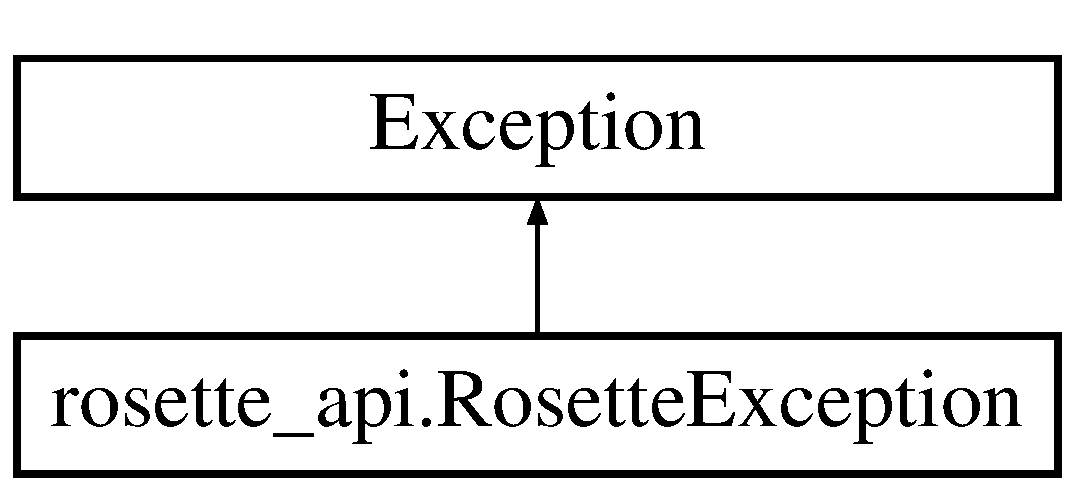
\includegraphics[height=2.000000cm]{classrosette__api_1_1_rosette_exception}
\end{center}
\end{figure}
\subsection*{Public Member Functions}
\begin{DoxyCompactItemize}
\item 
\hyperlink{classrosette__api_1_1_rosette_exception_a065c5e007dad0541bdfa7cab0400b6b0}{Rosette\+Exception} (string message=null, int code=0, string requestid=null, string file=null, string line=null)
\begin{DoxyCompactList}\small\item\em \hyperlink{classrosette__api_1_1_rosette_exception}{Rosette\+Exception} \end{DoxyCompactList}\end{DoxyCompactItemize}
\subsection*{Properties}
\begin{DoxyCompactItemize}
\item 
int \hyperlink{classrosette__api_1_1_rosette_exception_a2c6de2baf841c9b0453058968345b082}{Code}\hspace{0.3cm}{\ttfamily  \mbox{[}get, set\mbox{]}}
\begin{DoxyCompactList}\small\item\em Code \end{DoxyCompactList}\item 
string \hyperlink{classrosette__api_1_1_rosette_exception_a124d4746ae63df0352290ac841019163}{Request\+I\+D}\hspace{0.3cm}{\ttfamily  \mbox{[}get, set\mbox{]}}
\begin{DoxyCompactList}\small\item\em Request\+I\+D \end{DoxyCompactList}\item 
string \hyperlink{classrosette__api_1_1_rosette_exception_a060ff0690a35a0afbe15ecebe892a5a7}{File}\hspace{0.3cm}{\ttfamily  \mbox{[}get, set\mbox{]}}
\begin{DoxyCompactList}\small\item\em File \end{DoxyCompactList}\item 
string \hyperlink{classrosette__api_1_1_rosette_exception_a30a50a43d7edb20f3176ae4f048fa976}{Line}\hspace{0.3cm}{\ttfamily  \mbox{[}get, set\mbox{]}}
\begin{DoxyCompactList}\small\item\em Line \end{DoxyCompactList}\end{DoxyCompactItemize}


\subsection{Detailed Description}
\hyperlink{classrosette__api_1_1_rosette_exception}{Rosette\+Exception} Class 

\hyperlink{classrosette__api_1_1_rosette_exception}{Rosette\+Exception}\+: Custom exception to describe an exception from the Rosette A\+P\+I. 

\subsection{Constructor \& Destructor Documentation}
\hypertarget{classrosette__api_1_1_rosette_exception_a065c5e007dad0541bdfa7cab0400b6b0}{}\index{rosette\+\_\+api\+::\+Rosette\+Exception@{rosette\+\_\+api\+::\+Rosette\+Exception}!Rosette\+Exception@{Rosette\+Exception}}
\index{Rosette\+Exception@{Rosette\+Exception}!rosette\+\_\+api\+::\+Rosette\+Exception@{rosette\+\_\+api\+::\+Rosette\+Exception}}
\subsubsection[{Rosette\+Exception(string message=null, int code=0, string requestid=null, string file=null, string line=null)}]{\setlength{\rightskip}{0pt plus 5cm}rosette\+\_\+api.\+Rosette\+Exception.\+Rosette\+Exception (
\begin{DoxyParamCaption}
\item[{string}]{message = {\ttfamily null}, }
\item[{int}]{code = {\ttfamily 0}, }
\item[{string}]{requestid = {\ttfamily null}, }
\item[{string}]{file = {\ttfamily null}, }
\item[{string}]{line = {\ttfamily null}}
\end{DoxyParamCaption}
)}\label{classrosette__api_1_1_rosette_exception_a065c5e007dad0541bdfa7cab0400b6b0}


\hyperlink{classrosette__api_1_1_rosette_exception}{Rosette\+Exception} 

\hyperlink{classrosette__api_1_1_rosette_exception}{Rosette\+Exception}\+: Custom exception to describe an exception from the Rosette A\+P\+I. 


\begin{DoxyParams}{Parameters}
{\em message} & (string, optional)\+: Message describing exception details\\
\hline
{\em code} & (int, optional)\+: Code number of the exception\\
\hline
{\em requestid} & (string, optional)\+: Request\+I\+D if there is one\\
\hline
{\em file} & (string, optional)\+: Filename if in file\\
\hline
{\em line} & (string, optional)\+: Line if in file\\
\hline
\end{DoxyParams}


\subsection{Property Documentation}
\hypertarget{classrosette__api_1_1_rosette_exception_a2c6de2baf841c9b0453058968345b082}{}\index{rosette\+\_\+api\+::\+Rosette\+Exception@{rosette\+\_\+api\+::\+Rosette\+Exception}!Code@{Code}}
\index{Code@{Code}!rosette\+\_\+api\+::\+Rosette\+Exception@{rosette\+\_\+api\+::\+Rosette\+Exception}}
\subsubsection[{Code}]{\setlength{\rightskip}{0pt plus 5cm}int rosette\+\_\+api.\+Rosette\+Exception.\+Code\hspace{0.3cm}{\ttfamily [get]}, {\ttfamily [set]}}\label{classrosette__api_1_1_rosette_exception_a2c6de2baf841c9b0453058968345b082}


Code 

Getter, Setter for the Code Code\+: Code number of the exception Allows users to access the Exception Code \hypertarget{classrosette__api_1_1_rosette_exception_a060ff0690a35a0afbe15ecebe892a5a7}{}\index{rosette\+\_\+api\+::\+Rosette\+Exception@{rosette\+\_\+api\+::\+Rosette\+Exception}!File@{File}}
\index{File@{File}!rosette\+\_\+api\+::\+Rosette\+Exception@{rosette\+\_\+api\+::\+Rosette\+Exception}}
\subsubsection[{File}]{\setlength{\rightskip}{0pt plus 5cm}string rosette\+\_\+api.\+Rosette\+Exception.\+File\hspace{0.3cm}{\ttfamily [get]}, {\ttfamily [set]}}\label{classrosette__api_1_1_rosette_exception_a060ff0690a35a0afbe15ecebe892a5a7}


File 

Getter, Setter for the File File\+: Filename if in file Allows users to access the Exception File if in file \hypertarget{classrosette__api_1_1_rosette_exception_a30a50a43d7edb20f3176ae4f048fa976}{}\index{rosette\+\_\+api\+::\+Rosette\+Exception@{rosette\+\_\+api\+::\+Rosette\+Exception}!Line@{Line}}
\index{Line@{Line}!rosette\+\_\+api\+::\+Rosette\+Exception@{rosette\+\_\+api\+::\+Rosette\+Exception}}
\subsubsection[{Line}]{\setlength{\rightskip}{0pt plus 5cm}string rosette\+\_\+api.\+Rosette\+Exception.\+Line\hspace{0.3cm}{\ttfamily [get]}, {\ttfamily [set]}}\label{classrosette__api_1_1_rosette_exception_a30a50a43d7edb20f3176ae4f048fa976}


Line 

Getter, Setter for the Line Line\+: Line if in file Allows users to access the Exception Line if in file \hypertarget{classrosette__api_1_1_rosette_exception_a124d4746ae63df0352290ac841019163}{}\index{rosette\+\_\+api\+::\+Rosette\+Exception@{rosette\+\_\+api\+::\+Rosette\+Exception}!Request\+I\+D@{Request\+I\+D}}
\index{Request\+I\+D@{Request\+I\+D}!rosette\+\_\+api\+::\+Rosette\+Exception@{rosette\+\_\+api\+::\+Rosette\+Exception}}
\subsubsection[{Request\+I\+D}]{\setlength{\rightskip}{0pt plus 5cm}string rosette\+\_\+api.\+Rosette\+Exception.\+Request\+I\+D\hspace{0.3cm}{\ttfamily [get]}, {\ttfamily [set]}}\label{classrosette__api_1_1_rosette_exception_a124d4746ae63df0352290ac841019163}


Request\+I\+D 

Getter, Setter for the Request\+I\+D Request\+I\+D\+: Request\+I\+D if there is one Allows users to access the Exception Request\+I\+D 

The documentation for this class was generated from the following file\+:\begin{DoxyCompactItemize}
\item 
C\+A\+P\+I.\+cs\end{DoxyCompactItemize}

\hypertarget{classrosette__api_1_1_rosette_file}{}\section{rosette\+\_\+api.\+Rosette\+File Class Reference}
\label{classrosette__api_1_1_rosette_file}\index{rosette\+\_\+api.\+Rosette\+File@{rosette\+\_\+api.\+Rosette\+File}}


\hyperlink{classrosette__api_1_1_rosette_file}{Rosette\+File} Class  


\subsection*{Public Member Functions}
\begin{DoxyCompactItemize}
\item 
\hyperlink{classrosette__api_1_1_rosette_file_a979c8781846391dc237697e09423f472}{Rosette\+File} (string file, string data\+Type=\char`\"{}application/octet-\/stream\char`\"{}, string options=null)
\begin{DoxyCompactList}\small\item\em \hyperlink{classrosette__api_1_1_rosette_file}{Rosette\+File} \end{DoxyCompactList}\item 
string \hyperlink{classrosette__api_1_1_rosette_file_a92c60183e27f079750855b3aae00c58b}{get\+Filename} ()
\begin{DoxyCompactList}\small\item\em get\+Filename \end{DoxyCompactList}\item 
string \hyperlink{classrosette__api_1_1_rosette_file_af539cca8d69c0b71e46baed02987b3dc}{get\+Data\+Type} ()
\begin{DoxyCompactList}\small\item\em get\+Data\+Type \end{DoxyCompactList}\item 
byte\mbox{[}$\,$\mbox{]} \hyperlink{classrosette__api_1_1_rosette_file_a27511cf013b4cec685fe38cf8f6aa4d8}{get\+File\+Data} ()
\begin{DoxyCompactList}\small\item\em get\+File\+Data \end{DoxyCompactList}\item 
string \hyperlink{classrosette__api_1_1_rosette_file_aa7022b54ae4f9e6f42b66c0f6e0a6ad6}{get\+File\+Data\+String} ()
\begin{DoxyCompactList}\small\item\em get\+File\+Data\+String \end{DoxyCompactList}\item 
string \hyperlink{classrosette__api_1_1_rosette_file_add8db1d7668066dfcf4c7244fe791ed8}{get\+Options} ()
\begin{DoxyCompactList}\small\item\em get\+Options \end{DoxyCompactList}\end{DoxyCompactItemize}


\subsection{Detailed Description}
\hyperlink{classrosette__api_1_1_rosette_file}{Rosette\+File} Class 

\hyperlink{classrosette__api_1_1_rosette_file}{Rosette\+File}\+: Custom Datatype containing information about files for upload, and methods to read the files 

\subsection{Constructor \& Destructor Documentation}
\hypertarget{classrosette__api_1_1_rosette_file_a979c8781846391dc237697e09423f472}{}\index{rosette\+\_\+api\+::\+Rosette\+File@{rosette\+\_\+api\+::\+Rosette\+File}!Rosette\+File@{Rosette\+File}}
\index{Rosette\+File@{Rosette\+File}!rosette\+\_\+api\+::\+Rosette\+File@{rosette\+\_\+api\+::\+Rosette\+File}}
\subsubsection[{Rosette\+File(string file, string data\+Type=""application/octet-\/stream"", string options=null)}]{\setlength{\rightskip}{0pt plus 5cm}rosette\+\_\+api.\+Rosette\+File.\+Rosette\+File (
\begin{DoxyParamCaption}
\item[{string}]{file, }
\item[{string}]{data\+Type = {\ttfamily \char`\"{}application/octet-\/stream\char`\"{}}, }
\item[{string}]{options = {\ttfamily null}}
\end{DoxyParamCaption}
)}\label{classrosette__api_1_1_rosette_file_a979c8781846391dc237697e09423f472}


\hyperlink{classrosette__api_1_1_rosette_file}{Rosette\+File} 

\hyperlink{classrosette__api_1_1_rosette_file}{Rosette\+File}\+: Custom Datatype containing information about files for upload, and methods to read the files 


\begin{DoxyParams}{Parameters}
{\em file} & string\+: Path to the data file\\
\hline
{\em data\+Type} & (string, optional)\+: Description of the datatype of the data file. \char`\"{}application/octet-\/stream\char`\"{} is used if unsure.\\
\hline
{\em options} & (string, optional)\+: Json Options file to add extra information\\
\hline
\end{DoxyParams}


\subsection{Member Function Documentation}
\hypertarget{classrosette__api_1_1_rosette_file_af539cca8d69c0b71e46baed02987b3dc}{}\index{rosette\+\_\+api\+::\+Rosette\+File@{rosette\+\_\+api\+::\+Rosette\+File}!get\+Data\+Type@{get\+Data\+Type}}
\index{get\+Data\+Type@{get\+Data\+Type}!rosette\+\_\+api\+::\+Rosette\+File@{rosette\+\_\+api\+::\+Rosette\+File}}
\subsubsection[{get\+Data\+Type()}]{\setlength{\rightskip}{0pt plus 5cm}string rosette\+\_\+api.\+Rosette\+File.\+get\+Data\+Type (
\begin{DoxyParamCaption}
{}
\end{DoxyParamCaption}
)}\label{classrosette__api_1_1_rosette_file_af539cca8d69c0b71e46baed02987b3dc}


get\+Data\+Type 

get\+Data\+Type\+: Get the datatype 

\begin{DoxyReturn}{Returns}
string\+: String of the datatype
\end{DoxyReturn}
\hypertarget{classrosette__api_1_1_rosette_file_a27511cf013b4cec685fe38cf8f6aa4d8}{}\index{rosette\+\_\+api\+::\+Rosette\+File@{rosette\+\_\+api\+::\+Rosette\+File}!get\+File\+Data@{get\+File\+Data}}
\index{get\+File\+Data@{get\+File\+Data}!rosette\+\_\+api\+::\+Rosette\+File@{rosette\+\_\+api\+::\+Rosette\+File}}
\subsubsection[{get\+File\+Data()}]{\setlength{\rightskip}{0pt plus 5cm}byte \mbox{[}$\,$\mbox{]} rosette\+\_\+api.\+Rosette\+File.\+get\+File\+Data (
\begin{DoxyParamCaption}
{}
\end{DoxyParamCaption}
)}\label{classrosette__api_1_1_rosette_file_a27511cf013b4cec685fe38cf8f6aa4d8}


get\+File\+Data 

get\+File\+Data\+: Get the File\+Data in byte form 

\begin{DoxyReturn}{Returns}
byte\mbox{[}\mbox{]}\+: Byte Array of the file data
\end{DoxyReturn}
\hypertarget{classrosette__api_1_1_rosette_file_aa7022b54ae4f9e6f42b66c0f6e0a6ad6}{}\index{rosette\+\_\+api\+::\+Rosette\+File@{rosette\+\_\+api\+::\+Rosette\+File}!get\+File\+Data\+String@{get\+File\+Data\+String}}
\index{get\+File\+Data\+String@{get\+File\+Data\+String}!rosette\+\_\+api\+::\+Rosette\+File@{rosette\+\_\+api\+::\+Rosette\+File}}
\subsubsection[{get\+File\+Data\+String()}]{\setlength{\rightskip}{0pt plus 5cm}string rosette\+\_\+api.\+Rosette\+File.\+get\+File\+Data\+String (
\begin{DoxyParamCaption}
{}
\end{DoxyParamCaption}
)}\label{classrosette__api_1_1_rosette_file_aa7022b54ae4f9e6f42b66c0f6e0a6ad6}


get\+File\+Data\+String 

get\+File\+Data\+String\+: Get the File\+Data in string form 

\begin{DoxyReturn}{Returns}
string\+: String of the file data
\end{DoxyReturn}
\hypertarget{classrosette__api_1_1_rosette_file_a92c60183e27f079750855b3aae00c58b}{}\index{rosette\+\_\+api\+::\+Rosette\+File@{rosette\+\_\+api\+::\+Rosette\+File}!get\+Filename@{get\+Filename}}
\index{get\+Filename@{get\+Filename}!rosette\+\_\+api\+::\+Rosette\+File@{rosette\+\_\+api\+::\+Rosette\+File}}
\subsubsection[{get\+Filename()}]{\setlength{\rightskip}{0pt plus 5cm}string rosette\+\_\+api.\+Rosette\+File.\+get\+Filename (
\begin{DoxyParamCaption}
{}
\end{DoxyParamCaption}
)}\label{classrosette__api_1_1_rosette_file_a92c60183e27f079750855b3aae00c58b}


get\+Filename 

get\+Filename\+: Get the filename 

\begin{DoxyReturn}{Returns}
string\+: String of the filename
\end{DoxyReturn}
\hypertarget{classrosette__api_1_1_rosette_file_add8db1d7668066dfcf4c7244fe791ed8}{}\index{rosette\+\_\+api\+::\+Rosette\+File@{rosette\+\_\+api\+::\+Rosette\+File}!get\+Options@{get\+Options}}
\index{get\+Options@{get\+Options}!rosette\+\_\+api\+::\+Rosette\+File@{rosette\+\_\+api\+::\+Rosette\+File}}
\subsubsection[{get\+Options()}]{\setlength{\rightskip}{0pt plus 5cm}string rosette\+\_\+api.\+Rosette\+File.\+get\+Options (
\begin{DoxyParamCaption}
{}
\end{DoxyParamCaption}
)}\label{classrosette__api_1_1_rosette_file_add8db1d7668066dfcf4c7244fe791ed8}


get\+Options 

get\+Options\+: Get the options 

\begin{DoxyReturn}{Returns}
string\+: String of the options
\end{DoxyReturn}


The documentation for this class was generated from the following file\+:\begin{DoxyCompactItemize}
\item 
C\+A\+P\+I.\+cs\end{DoxyCompactItemize}

%--- End generated contents ---

% Index
\backmatter
\newpage
\phantomsection
\clearemptydoublepage
\addcontentsline{toc}{chapter}{Index}
\printindex

\end{document}
